\documentclass[11pt]{tg_usta}
% Informe TALLER-4 — Recuperación de Información sobre el corpus de la Comisión de la Verdad (CEV)
% Plantilla tg_usta (PUJ) adaptada del informe del TALLER-2 del mismo repositorio.
\usepackage{tcolorbox}
\usepackage{float}
\usepackage{graphicx}
\usepackage{makecell}
\usepackage{anysize}
\usepackage{cite} % para contraer referencias
\marginsize{1in}{1in}{1in}{1in} %% Márgenes NO MODIFICAR
\raggedbottom
\setlength{\textfloatsep}{8pt plus 2pt minus 4pt}
\setlength{\intextsep}{8pt plus 2pt minus 4pt}
\setlength{\abovecaptionskip}{4pt}
\setlength{\belowcaptionskip}{2pt}
\renewcommand{\topfraction}{0.9}
\renewcommand{\bottomfraction}{0.8}
\renewcommand{\textfraction}{0.07}
\renewcommand{\floatpagefraction}{0.75}
% Cargar los paquetes necesarios aquí
\usepackage{amsmath,amsthm,amssymb}
\usepackage{multicol}
\usepackage{url}
\usepackage{multirow}
\usepackage{tikz}
\usepackage[T1]{fontenc}
\usepackage{array}
\usepackage{booktabs}
\usetikzlibrary{trees}
\usepackage{xurl}
\setlength{\emergencystretch}{1.5em}
\renewcommand{\tablename}{Tabla}
\usepackage[utf8]{inputenc}
\usepackage{subcaption}
\usepackage{listings}

\newtheorem{definicion}{Definición}[section]
\newtheorem{nota}{Nota}[section]
\newtheorem{problema}{Problema}[section]
\newtheorem{teorema}{Teorema}[section]
\newtheorem{corolario}{Corolario}[section]
\newtheorem{proposicion}{Proposición}[section]
\newtheorem{lema}{Lema}[section]
\allowdisplaybreaks
\decimalpoint

\lstset{
    basicstyle=\ttfamily\scriptsize,
    breaklines=true,
    frame=single,
    columns=fullflexible,
    keepspaces=true,
    showstringspaces=false,
    captionpos=b,
    numbers=left,
    numberstyle=\tiny,
    xleftmargin=1.5em
}

\sloppy
\begin{document}
\title[maintitle = Recuperación de Información aplicada a entrevistas y libros de la Comisión de la Verdad,
       secondtitle = Taller 4 - Procesamiento de Lenguaje Natural]

\begin{authors}[Rivera, Carrillo, Garnica \& Prieto]

\author[affiliation = PUJ,
        firstname = Erika Valeria,
        surname = Rivera Jiménez,
        email = riveraev@javeriana.edu.co]

\author[affiliation = PUJ,
        firstname = Julián Guillermo,
        surname = Carrillo Meneses,
        email = carrillojuliang@javeriana.edu.co]

\author[affiliation = PUJ,
        firstname = Carlos Andrés,
        surname = Garnica Salazar,
        email = carlos\_garnicas@javeriana.edu.co]

\author[affiliation = PUJ,
        firstname = Oscar Andrés,
        surname = Prieto Moreno,
        email = o-prieto@javeriana.edu.co]

\end{authors}

\begin{mainabstract}

Este informe final integra los seis puntos del taller de Recuperación de Información (IR) sobre el corpus de la Comisión de la Verdad (CEV) y documenta, para cada uno, tanto el procedimiento seguido como la justificación de sus decisiones metodológicas. Se extrajeron \textbf{917 segmentos} de los 10 tomos del Informe Final (2.271.493 palabras; mapeo del TOC 91-100\,\%, cobertura 100\,\%) y se normalizaron y preprocesaron \textbf{2.486 entrevistas} CEV/JEP (200,5 M de caracteres $\rightarrow$ 188,8 M, $-5{,}82$\,\%; 40,35 M de tokens $\rightarrow$ 10,92 M de lemas). El análisis exploratorio evidenció un desajuste de registro (Jaccard de vocabulario 0,221; TTR$_{m1000}$ 0,609 libros vs. 0,514 entrevistas; Yule K 31,8 vs. 38,7) y 345 pares casi idénticos ($>$0,85) que se conservan por integridad del corpus. El modelo TF-IDF (118.748 features con bigramas, tf sublineal y norma l2) alcanza una cobertura del 99,92\,\% y, sobre una muestra etiquetada de 30 pares, P@1 de 0,533 (estricto) y 1,0 (aceptable). Okapi BM25 (k$_1$=1,5; b=0,75) y Rocchio (con retroalimentación por pseudo-relevancia, $\alpha$=1, $\beta$=0,75, $\gamma$=0,15), implementados manualmente desde cero con auto-verificaciones sintéticas en verde, comparten la señal del modelo base (57,0\,\% y 70,1\,\% de top-1 idéntico) y confirman el sesgo de dominio hacia el tomo TESTIMONIAL (76,77\,\%, 75,0\,\% y 78,4\,\%). La comparación de corpus mediante un heatmap agregado 10$\times$10 (diagonal media 0,0725 $>$ 0,0608 fuera de la diagonal), un heatmap top-25 por documento y un cuadro de 30 vínculos con fragmentos cierra el proceso con evidencia trazable y límites declarados.
 \textit{\textbf{Palabras clave:}} Recuperación de Información, TF-IDF, Okapi BM25, Rocchio, Comisión de la Verdad, Procesamiento de Lenguaje Natural
 \end{mainabstract}


\section{Introducción}

El taller propone desarrollar un proceso de Recuperación de Información (IR) que determine qué entrevistas del registro oral de la Comisión de la Verdad (CEV) se relacionan con testimonios o secciones de los libros del Informe Final, y que mida la relevancia de esos vínculos con métricas explícitas. El problema plantea un desajuste de registro poco habitual en IR: las consultas son habla oral transcrita y anotada, mientras que la colección es prosa académica institucional. El corpus de consultas lo constituyen \textbf{2.486 entrevistas} CEV/JEP y la colección a recuperar quedó conformada por \textbf{917 segmentos} extraídos de los \textbf{10 tomos} del Informe Final \cite{cev2022informe}. La pregunta que articula el informe es doble: \textit{¿cómo relacionar dos registros tan distintos ---oral transcrito y escrito académico--- y qué aporta cada familia de métricas a la lectura de esos vínculos?}

Metodológicamente, el trabajo sigue el orden del enunciado y cada componente se documenta con su procedimiento, sus parámetros y la evidencia que respalda cada decisión: \textbf{(P1)} extracción y preparación del corpus, con definición explícita de la morfología documental; \textbf{(P2)} análisis exploratorio del corpus (estadísticas, diversidad léxica, nubes, comparación léxica y near-duplicados); \textbf{(P3)} modelo de IR con vectorización TF-IDF y similitud coseno; \textbf{(P4)} implementación manual de Okapi BM25 y Rocchio con comparación de sus rankings; \textbf{(P5)} comparación de corpus mediante heatmap y cuadro de vínculos; y \textbf{(P6)} este informe final, que incluye la evaluación crítica y las mejoras futuras. Todos los artefactos intermedios ---segmentos, corpus normalizados, rankings, figuras y tablas--- se generan de forma determinista y quedan trazables en el repositorio.

El estado del arte condiciona el diseño. La literatura computacional sobre el corpus CEV es inexistente; el trabajo más cercano es la minería de textos y redes lingüísticas sobre audiencias públicas de la JEP \cite{sosa2025constructing}, que valida la viabilidad del análisis léxico de narrativas de víctimas del conflicto colombiano. Desde las humanidades, el análisis del volumen testimonial de la CEV \cite{castillejo2023escuchar} fundamenta una decisión de diseño central: la oralidad no es solo ruido que limpiar, sino un rasgo constitutivo del género. En IR en español, MessIRve \cite{valentini2024messirve} muestra que los modelos léxicos siguen siendo una línea base competitiva, lo que respalda la elección de TF-IDF \cite{salton1988term} y de sus extensiones probabilísticas \cite{robertson2009probabilistic} como núcleo del taller.

De ese estado del arte se desprende la consecuencia metodológica más importante: \textbf{no existe un gold estándar} para este tipo de vínculo, de modo que la evaluación se plantea como cualitativa sobre una muestra etiquetada por el equipo y como acuerdo entre rankings, y así se declara de forma explícita en todo el informe. Esta limitación, asumida desde el diseño, explica que el trabajo priorice la trazabilidad y la reproducibilidad sobre la comparación contra una referencia externa que no está disponible.


\section{Datos y consideraciones éticas}\label{sec:datos}

\subsection{Los tres insumos}

\textbf{Entrevistas.} El archivo \texttt{data/raw/entrevistas\_all\_2023-03-21\_14-24\_05.json} (231 MB) contiene \textbf{2.486 registros} \texttt{\{id\_doc, pages, text\}} del registro oral CEV/JEP. Se trata de transcripciones ya anonimizadas por la Comisión mediante marcas en mayúsculas con numeración (\texttt{LUGAR1}, \texttt{FAMILIAR2}, \texttt{ORGANIZACION PUBLICA 1}, etc.), anotaciones de transcripción (interrupciones, pasajes dudosos, risas, llanto) y etiquetas de hablante (\texttt{ENT:}, \texttt{TEST:}). La extensión es extremadamente asimétrica ---entre 3 y 850 mil caracteres en crudo, con media de 3.902,9 lemas de contenido por entrevista frente a una mediana de 3.112,5 (p99 $\approx$ 20.282)---, lo que obliga a controlar la longitud en cualquier comparación léxica y anticipa dos decisiones metodológicas: medir la diversidad con muestras de tamaño fijo y evaluar el ranking sobre medias y percentiles en lugar de totales (Sección~\ref{sec:p2}).

\textbf{Libros.} La colección la conforman los 10 tomos del Informe Final en PDF, que ocupan 301 MB extraídos y \textbf{6.144 páginas}: HALLAZGOS, CONVOCATORIA, NARRATIVA, SUFRIR, TESTIMONIAL, CUERPO, NNA, VIOLACIONES, ETNICO y FUERA. La heterogeneidad de tamaños y de temas entre tomos es una propiedad del Informe y condiciona el diseño: el tomo testimonial (680 páginas) reproduce el registro oral de las víctimas y resultó determinante en el comportamiento del modelo (Sección~\ref{sec:p3}), de modo que su influencia se documenta y se mide en lugar de asumirse.

\textbf{Tesauro.} \texttt{data/raw/Resource-tesauro.rdf} ($\approx$5 MB, SKOS, 10.151 etiquetas en español) es el vocabulario controlado de la CEV. \textbf{No se integra al modelo}: se evaluaron dos alternativas y ambas se descartaron. Filtrar el vocabulario del IR con términos controlados habría empobrecido el matching, porque el tesauro no cubre el habla oral de las entrevistas; expandir las consultas con sinónimos SKOS habría quedado fuera del alcance del modelo léxico y, al no existir gold estándar, no habría forma de medir si el beneficio compensaba la complejidad añadida. El recurso se aprovecha de forma cualitativa en el EDA (Sección~\ref{sec:p2}), donde se verifica si sus etiquetas iluminan los términos distintivos de cada corpus.

\subsection{Ética y tratamiento de datos sensibles}

El corpus contiene narrativas de víctimas, por lo que la documentación de procedencia y contexto sigue los \textit{data statements} de Bender y Friedman \cite{bender2018data} y el patrón de construcción de corpus en español de Puertas et al. \cite{puertas2018automatic}. Ese compromiso se materializa en tres decisiones verificables. Primero, \textbf{no se re-identifica a ninguna persona}: la normalización de anonimizados a categorías canónicas conserva el papel semántico del referente (lugar, familiar, organización) sin publicar sus identificadores, y la categorización se declara como una transformación interna del corpus y no como un intento de recuperar identidades. Segundo, la auditoría de privacidad verificó presencia de PII hablada en el intermedio local \texttt{entrevistas\_normalizadas.jsonl} (1 cédula, 2 celulares, 118 corridas de 6-10 dígitos y 1.773 tokens UPPER+dígito pegados, del tipo \texttt{CONOCIDO9lo}); \textbf{los corpus finales y todos los resultados publicados están limpios} (0 correos, 0 cédulas, 0 teléfonos, 0 tokens UPPER+dígito), porque el filtro lingüístico del preprocesado los elimina en una segunda etapa. Tercero, \texttt{data/raw/} permanece intacto: el pipeline lee los insumos pero nunca los reescribe, de modo que cualquier auditoría puede repetirse sobre la fuente original.

A lo anterior se suma una decisión de integridad: los 345 pares de entrevistas casi idénticas detectados en el EDA \textbf{no se eliminan} (Sección~\ref{sec:p2}). Se documentan porque duplican rankings y sobreestiman la cobertura, pero se prefirió conservar el corpus oficial íntegro antes que introducir un filtrado no solicitado que alterara su composición. Finalmente, el notebook que acompaña este informe es reproducible con \textbf{solo 3 insumos descargados manualmente} (entrevistas, libros y tesauro); todo lo demás ---segmentos, normalizadas, lemas, rankings, figuras--- lo genera el propio notebook, de modo que la distribución del material no requiere compartir datos derivados con PII y la cadena completa puede auditarse desde las fuentes.


\section{P1 --- Extracción y preparación del corpus}\label{sec:p1}

\subsection{Morfología del documento a recuperar}

Antes de extraer nada hubo que decidir \textit{qué} es un documento. En IR vectorial esa decisión no está dada por el formato: si el documento fuera el tomo completo, la similitud se diluiría entre decenas de temas; si fuera la página, los vectores serían pobres y romperían unidades temáticas; si fuera el párrafo, resultarían demasiado cortos para una estimación estable de pesos. La morfología adoptada quedó fijada en dos niveles. La \textbf{colección} son \textbf{segmentos de tomo}: secciones del TOC con granularidad de \textbf{niveles 1-2 según el tomo} (nivel 2 cuando existe; nivel 1 si el TOC es plano). Las secciones de menos de 300 palabras se fusionan con la siguiente (o la anterior si es la última de su padre), porque un fragmento tan corto aporta pocos términos y genera un vector inestable; las de más de 4.000 palabras sin subsecciones se dividen en fragmentos de hasta 3.500 palabras cortando en límite de párrafo o de página, para no mezclar temas ni romper la prosa; portada, catálogo editorial, comisionados, TOC, bibliografía, glosario, anexos y créditos se descartan por no contener materia temática comparable con los testimonios. Cada segmento se identifica con el esquema \texttt{TOMO\_abrev-p<página\_inicio>-<titulo\_normalizado>} y conserva metadatos \texttt{\{id\_segmento, tomo, titulo, nivel\_toc, pagina\_inicio, pagina\_fin, n\_palabras, texto\}}, lo que permite auditar de dónde salió cada unidad. Las \textbf{queries} son la transcripción completa de cada \texttt{id\_doc} con sus metadatos \texttt{\{id\_doc, pages\}}. La banda objetivo de 300-4.000 palabras equilibra especificidad y robustez del vector; la media final fue de 2.477 palabras por segmento, dentro del rango previsto.

\subsection{Pipeline de extracción de libros}

El script \texttt{scripts/01\_extraer\_libros.py} implementa cinco etapas encadenadas. (i) La conversión página a página con \texttt{pdftotext -layout} en 32 hilos preserva la disposición espacial del texto, necesaria para reconstruir encabezados y tablas. (ii) El parser del TOC por tomo combina sangrado, coordenadas \texttt{x0} de PyMuPDF y paridad de márgenes para reconstruir la jerarquía sin depender de un único indicio, dado que los TOC del Informe no son uniformes. (iii) Antes de mapear títulos se calibra el desfase entre página impresa y página del PDF (verificado \textbf{offset = 0} en TESTIMONIAL); sin esta verificación, un desplazamiento constante asignaría a cada sección el texto de la página contigua. (iv) El matching del título normalizado contra los encabezados del cuerpo se hace en una ventana de página $\pm$1 para tolerar títulos que abren en la página siguiente o que aparecen con variaciones mínimas. (v) Una \textit{blacklist} automática de encabezados y pies repetidos (\textit{running heads}) evita confundir esos rótulos con títulos de sección. Los controles de sanidad exigidos por la arquitectura se cumplieron en los 10 tomos: mapeo del TOC $\geq$85\,\% (rango obtenido 91,2-100\,\%), cobertura de páginas de contenido $\geq$90\,\% (100\,\% en todos), 0 solapamientos, 0 segmentos vacíos y 0\,\% de segmentos fuera de banda. Esos umbrales se fijaron como garantía de cobertura razonable manteniendo la extracción automática: un mapeo inferior al 85\,\% habría exigido revisión manual del tomo.

\begin{table}[htbp]
    \centering
    \caption{Segmentos extraídos por tomo del Informe Final CEV. Fuente: \texttt{resultados/extraccion\_libros\_report.json}.}
    \footnotesize
    \setlength{\tabcolsep}{4pt}
    \begin{tabular}{l r r r r}
    \toprule
    Tomo & Páginas PDF & Segmentos & Palabras & Mapeo TOC \\
    \midrule
    VIOLACIONES & 1.144 & 148 & 457.293 & 100,0\,\% \\
    HALLAZGOS   & 792   & 146 & 309.169 & 100,0\,\% \\
    NARRATIVA   & 656   & 111 & 230.995 & 98,1\,\% \\
    TESTIMONIAL & 680   & 104 & 271.338 & 100,0\,\% \\
    FUERA       & 548   & 96  & 211.824 & 100,0\,\% \\
    ETNICO      & 752   & 91  & 286.607 & 100,0\,\% \\
    CUERPO      & 644   & 84  & 188.189 & 95,3\,\% \\
    SUFRIR      & 484   & 68  & 161.620 & 96,1\,\% \\
    NNA         & 388   & 55  & 140.301 & 91,2\,\% \\
    CONVOCATORIA& 56    & 14  & 14.157  & 100,0\,\% \\
    \midrule
    \textbf{Total} & \textbf{6.144} & \textbf{917} & \textbf{2.271.493} & 91,2-100\,\% \\
    \bottomrule
    \end{tabular}
    \label{tab:segmentos}
\end{table}

\begin{figure}[htbp]
    \centering
    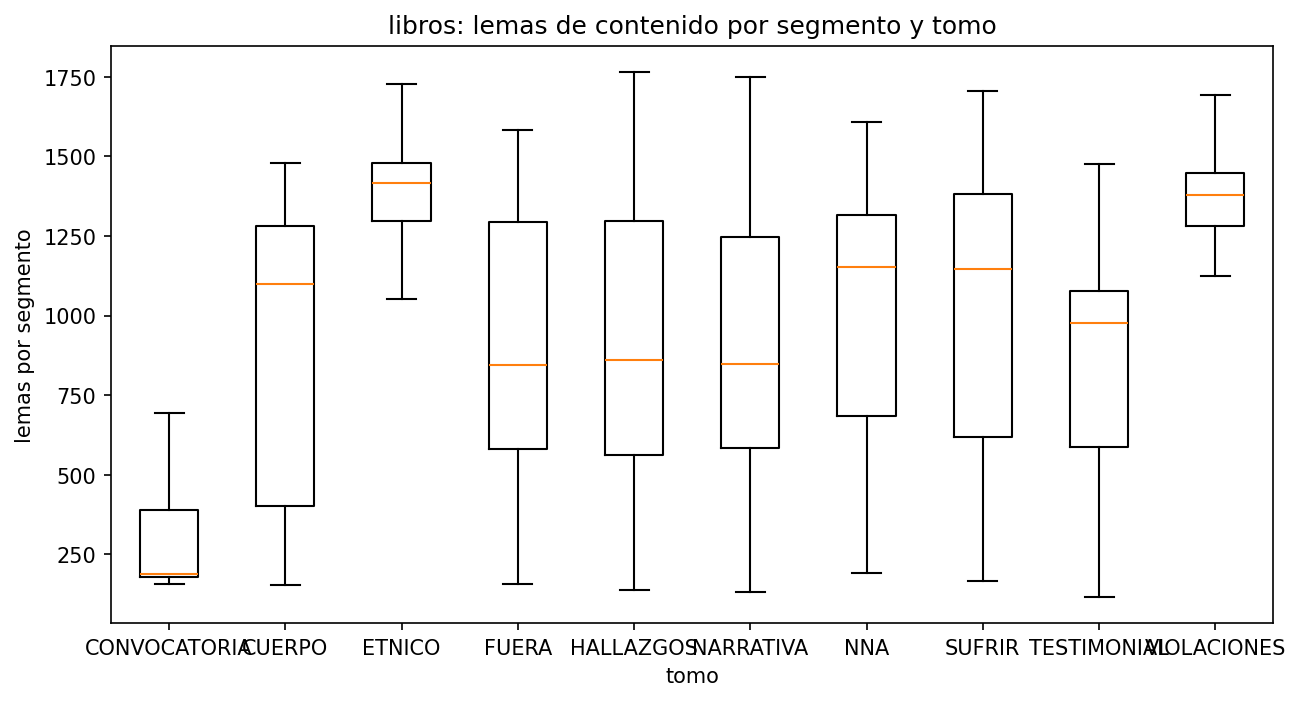
\includegraphics[width=0.62\textwidth]{figuras/eda_libros_lemas_por_tomo.png}
    \caption{Lemas de contenido por tomo tras el preprocesado. La distribución muestra que VIOLACIONES y HALLAZGOS concentran el mayor volumen léxico, mientras CONVOCATORIA es un tomo pequeño (14.157 palabras en 14 segmentos). Conclusión: la colección cubre el ciclo completo del conflicto con tamaños heterogéneos, lo que obliga a comparar afinidades medias por par y no masas totales en el heatmap (Sección~\ref{sec:p5}).}
    \label{fig:lemas-tomo}
\end{figure}

\subsection{Normalización estructural de entrevistas}

Las transcripciones no son texto plano: contienen códigos de sistema, anotaciones y marcas de anonimización. La normalización regex se ejecutó por etapas separadas en 58,4 s con un pico de 679,9 MB de RAM y redujo el corpus de \textbf{200.518.396 a 188.838.879 caracteres} ($-5{,}82$\,\%). Se eliminaron 422 códigos líder, 604 líneas \texttt{AUDIO}, 896 códigos embebidos, 138.613 anotaciones entre corchetes (\texttt{[INTERRUP]}, \texttt{[DUD: ...]}, \texttt{[risas]}, \texttt{[llanto]}), 653.328 etiquetas de hablante y 291.868 guiones. Separar la limpieza en etapas ---en lugar de una única expresión regular monolítica--- permitió contabilizar el aporte de cada transformación y verificar que ninguna eliminara contenido sustantivo. La decisión central fue \textbf{mapear los anonimizados a 8 categorías canónicas} en minúsculas, en lugar de eliminarlos o dejarlos como estaban: eliminarlos habría borrado vocabulario con papel semántico relevante para el matching (``mi familiar desapareció'' conecta con las secciones sobre desaparición de familiares), mientras que conservar \texttt{LUGAR1}, \texttt{LUGAR2} o \texttt{FAMILIAR3} tal cual fragmenta el vocabulario en tipos triviales. Las categorías canónicas se comportan como un solo token léxico ---420 variantes ortográficas se reducen a 8 patrones--- y se preservan a lo largo de todo el pipeline, de modo que el modelo puede explotar el papel del referente sin exponer su identidad.

\begin{table}[htbp]
    \centering
    \caption{Anonimizados de entrevistas normalizados a categorías canónicas (8 patrones, 420 variantes ortográficas). Fuente: \texttt{resultados/metricas.json}, fase 4.}
    \small
    \setlength{\tabcolsep}{6pt}
    \begin{tabular}{l r}
    \toprule
    Categoría canónica & Ocurrencias \\
    \midrule
    \texttt{conocido} & 58.525 \\
    \texttt{anonimo} (genérico) & 43.262 \\
    \texttt{organizacion\_social} & 25.336 \\
    \texttt{lugar} & 24.226 \\
    \texttt{familiar} & 21.428 \\
    \texttt{organizacion\_publica} & 18.878 \\
    \texttt{institucion\_educativa} & 5.974 \\
    \texttt{partido\_politico} & 1 \\
    \midrule
    \textbf{Total mapeado} & \textbf{197.630} \\
    \bottomrule
    \end{tabular}
    \label{tab:anonimizados}
\end{table}

\subsection{Preprocesado lingüístico}

El preprocesado aplica un pipeline único de spaCy \texttt{es\_core\_news\_md} \cite{spacy2024model} a ambos corpus: tokenización, minúsculas, lematización y parada \textit{en consumo}. Se eligió lematización sobre \textit{stemming} porque los stems del español sobre-fusionan formas (``paz/pacer'') y porque el lematizador de spaCy es el estándar práctico para español; además, el vocabulario unificado de lemas es lo que permite comparar el registro oral con el escrito, y se descartó el modelo grande \texttt{es\_core\_news\_lg} por no aportar ventaja relevante para lematización a un costo mayor. La lista de parada combina \textbf{521 stopwords de spaCy + 51 muletillas del habla colombiana + 42 tokens de ruido tipográfico de los libros} (p.~ej.\ palabras partidas por guion, \texttt{ibid.}), para un total efectivo de \textbf{611 tokens}; las muletillas (\textit{eh, mmm, este, o sea, pues}) no provienen de una lista genérica, sino que se detectaron empíricamente en las frecuencias del corpus, y su tratamiento se apoya en la caracterización del español colombiano de Moreno-Sandoval et al. \cite{moreno2024detection}. La parada se aplica \textit{en consumo}: los textos normalizados conservan todos los tokens y el filtrado ocurre en cada uso, de modo que distintas métricas pueden recalcularse con o sin parada sin volver a procesar el corpus. Adicionalmente se aplicaron \textbf{62 correcciones de lemas} en consumo (\texttt{atreveír}$\rightarrow$\texttt{atrever}, voseo, truncamientos orales), se conservaron los años de 4 dígitos en rango 1900-2025 y las categorías canónicas como tokens únicos, y se descartaron tokens no alfabéticos y de un carácter.

La producción fue determinista y reanudable (checkpoint por documento): libros 917 documentos en 30,5 s; entrevistas 2.486 en $\approx$509,5 s (4,88 documentos/s). El resultado son \textbf{40.346.344 tokens crudos y 10.923.423 lemas} en entrevistas (ratio 0,2707), de los cuales quedan 9.702.534 lemas de contenido tras la parada; 2 entrevistas quedan legítimamente vacías (sus textos normalizados de origen están vacíos) y se documentan sin eliminarlas, porque su exclusión alteraría el denominador de la cobertura. El corpus resultante es \texttt{data/corpus/segmentos\_libros.jsonl} (917), \texttt{entrevistas\_normalizadas.jsonl} (2.486) y \texttt{preprocesado/\{libros,entrevistas\}\_\{lemas,tokens\}.txt} más los \texttt{*\_docs.json}. La calidad técnica se verificó con ruff (0 errores) y 51 pruebas pytest aprobadas, y la ejecución por lotes con punto de control permite reanudar sin recomputar lo ya procesado.

\subsection{Síntesis de decisiones y controles de calidad}

El punto 1 concentra las decisiones que condicionan todo el taller, y cada una se tomó con una alternativa explícita sobre la mesa: el documento a recuperar es una sección temática (nivel 1-2 del TOC) y no un tomo, una página o un párrafo; las secciones cortas se fusionan y las muy largas se fragmentan para mantener la banda 300-4.000 palabras; los anonimizados se mapean a 8 categorías canónicas en lugar de eliminarse o dejarse crudos; el texto se lematiza con spaCy en lugar de stems, y la parada ---base de spaCy más muletillas empíricas y ruido tipográfico--- se aplica en consumo. El control de esas decisiones no depende de inspección manual: los 10 tomos pasaron los umbrales de mapeo y cobertura, la normalización reportó el conteo de cada transformación, el pipeline es determinista y reanudable, y el código quedó cubierto por 51 pruebas automáticas y análisis estático sin errores. En conjunto, el punto 1 no solo produce los insumos de P2-P5, sino que fija y documenta la morfología sobre la que se calculan todas las métricas posteriores.


\section{P2 --- Análisis exploratorio del corpus}\label{sec:p2}

\subsection{Estadísticas descriptivas y control de la longitud}

El EDA se ejecutó sobre 917 segmentos de libro y 2.486 entrevistas con el corpus lematizado y con la parada aplicada en consumo. La Tabla~\ref{tab:eda-stats} resume las cifras. La conclusión estructural es la \textbf{asimetría de longitudes}: las entrevistas promedian 3.902,9 lemas de contenido pero su mediana es 3.112,5 y su extremo superior supera los 45.000, mientras los segmentos de libro son mucho más homogéneos (media 1.012,3; máximo 1.765). Por eso el análisis reporta media, mediana y percentiles en lugar de totales, y por eso cualquier métrica de riqueza léxica sin control de longitud estaría midiendo el tamaño del documento, no su diversidad. Esta observación no es un detalle descriptivo: es la que fija las reglas de comparación del resto del taller.

\begin{table}[htbp]
    \centering
    \caption{Estadísticas del corpus preprocesado (lemas de contenido, parada en consumo). Fuente: \texttt{resultados/eda/estadisticas\_corpus.csv} y \texttt{metricas.json}, fase 5.}
    \small
    \setlength{\tabcolsep}{5pt}
    \begin{tabular}{l r r}
    \toprule
    Métrica & Libros (917) & Entrevistas (2.486) \\
    \midrule
    Tokens crudos spaCy & 2.624.040 & 40.346.344 \\
    Lemas de contenido & 928.253 & 9.702.534 \\
    Tipos (vocabulario) & 33.277 & 109.391 \\
    Media de lemas/doc & 1.012,3 & 3.902,9 \\
    Mediana de lemas/doc & 1.124,0 & 3.112,5 \\
    TTR con muestra fija n=1.000 & \textbf{0,609} & 0,514 \\
    Yule K (menor = más diverso) & \textbf{31,8} & 38,7 \\
    \bottomrule
    \end{tabular}
    \label{tab:eda-stats}
\end{table}

\begin{figure}[htbp]
    \centering
    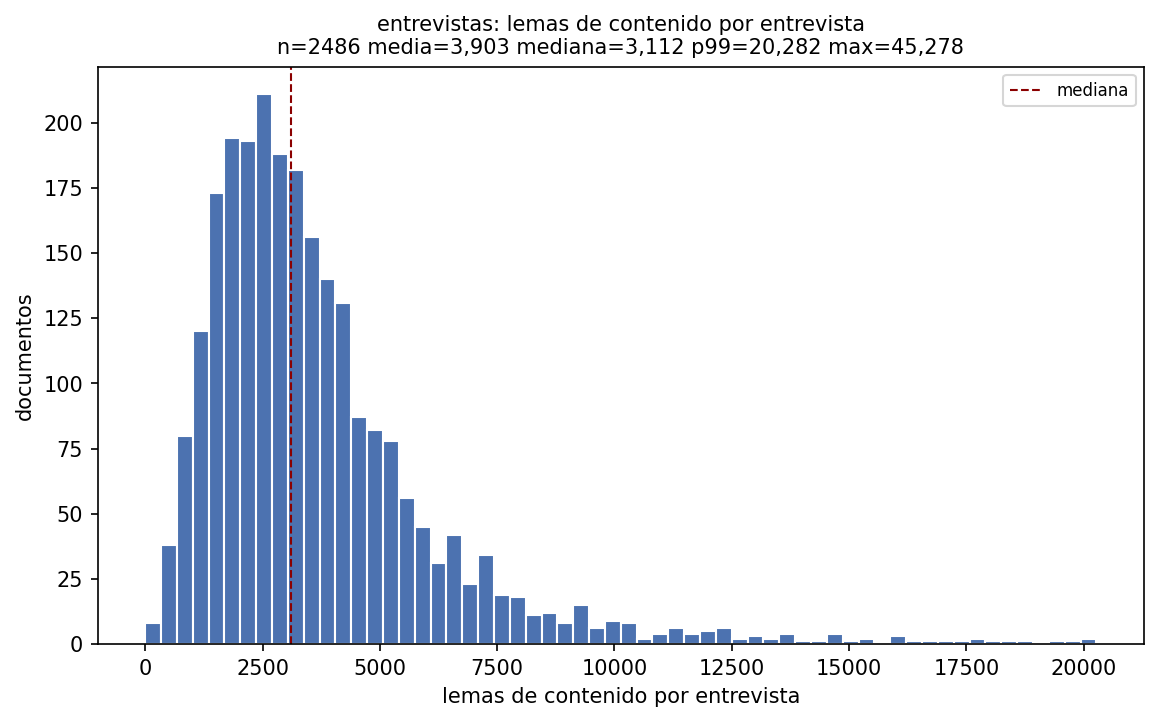
\includegraphics[width=0.54\textwidth]{figuras/eda_entrevistas_hist_lemas.png}
    \caption{Histograma de lemas de contenido por entrevista. La cola derecha (entrevistas de decenas de miles de lemas) convive con documentos cortos y 2 vacíos legítimos. Conclusión: la distribución es fuertemente asimétrica, por lo que el TTR se midió con muestras de tamaño fijo y la evaluación se reportó sobre medias y percentiles, no sobre totales.}
    \label{fig:hist-lemas-entrevistas}
\end{figure}

\begin{figure}[htbp]
    \centering
    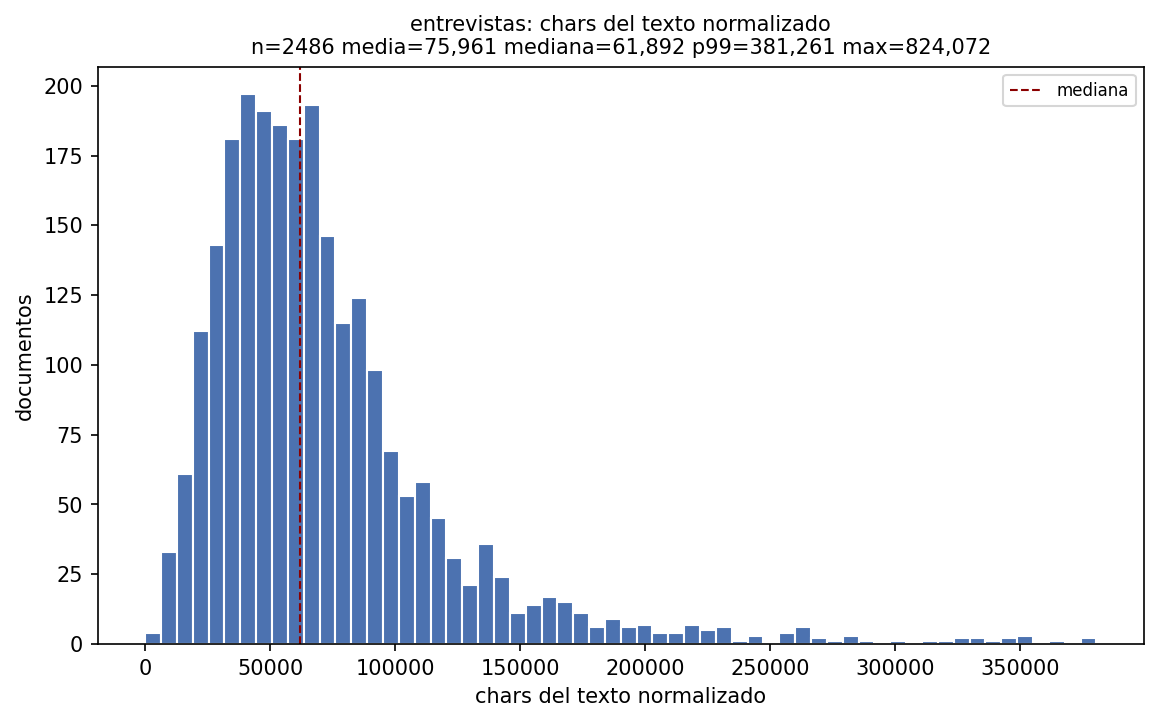
\includegraphics[width=0.54\textwidth]{figuras/eda_entrevistas_hist_chars.png}
    \caption{Histograma de caracteres normalizados por entrevista (rango 0-824.072; el crudo llegaba a 850 mil). Conclusión: la normalización estructural redujo el 5,82\,\% de los caracteres sin tocar el contenido testimonial, y la asimetría extrema de origen se conserva, lo que justifica las decisiones de robustez (lemas, parada y evaluación por muestras) del resto del taller.}
    \label{fig:hist-chars-entrevistas}
\end{figure}

\begin{figure}[htbp]
    \centering
    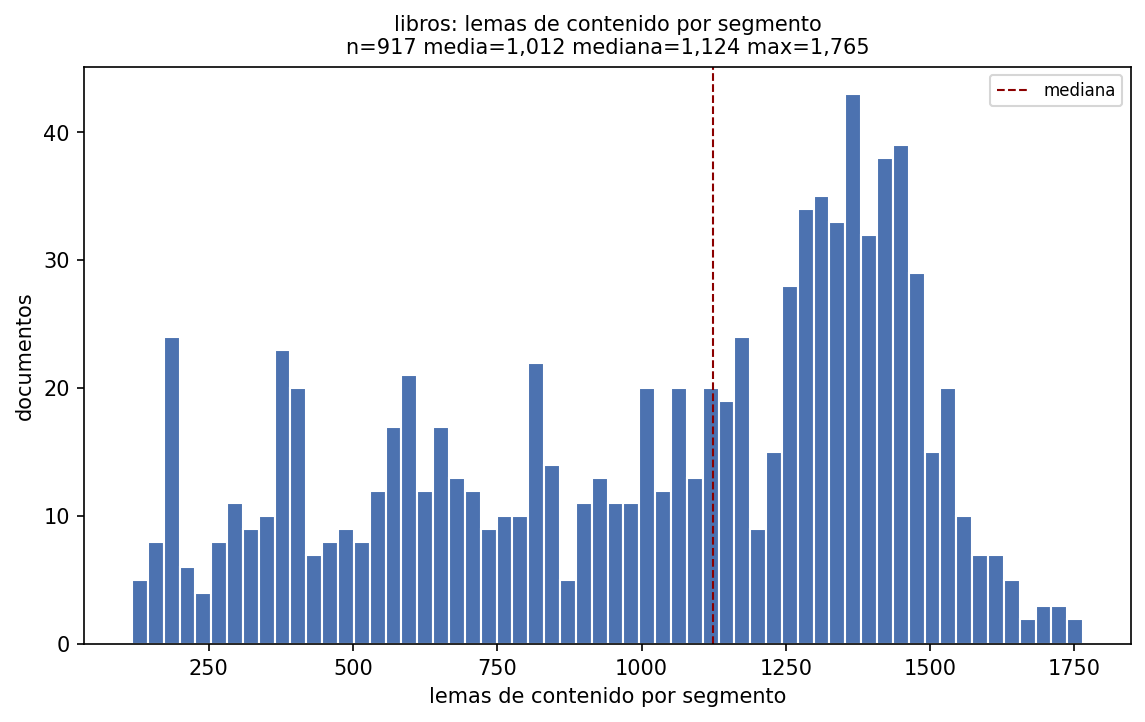
\includegraphics[width=0.55\textwidth]{figuras/eda_libros_hist_lemas.png}
    \caption{Histograma de lemas de contenido por segmento de libro. A diferencia de las entrevistas, la distribución es compacta y centrada en torno a 1.000 lemas. Conclusión: la granularidad TOC niveles 1-2 produjo unidades de tamaño comparable, condición necesaria para que la similitud coseno no esté dominada por el tamaño del documento.}
    \label{fig:hist-libros}
\end{figure}

\subsection{Diversidad léxica}

Como el TTR depende de la longitud (el ``problema doble'' de Bestgen \cite{bestgen2023measuring}), la diversidad se midió con \textbf{TTR de muestra fija (n=1.000)} y con el índice \textbf{Yule K} sobre el documento completo, cuyo menor valor indica mayor diversidad. Se eligieron ambos índices por complementariedad: el TTR muestreado reduce todos los documentos a la misma ventana de 1.000 tokens y, por tanto, es comparable entre longitudes; Yule K es un índice global que mide la concentración de frecuencia de tipos y no requiere truncar el documento. Los libros resultaron más diversos (\textbf{TTR$_{m1000}$ 0,609 vs. 0,514; Yule K 31,8 vs. 38,7}). La lectura es consistente con la naturaleza de cada registro: el texto académico explota un vocabulario institucional y analítico amplio, mientras la oralidad transcrita es más repetitiva, con alta frecuencia de verbos de narración y de referencias genéricas, algo esperable en habla espontánea y documentado para el español colombiano \cite{moreno2024detection}. Que ambos índices coincidan en la misma dirección respalda que la brecha de registro es una propiedad del corpus y no un artefacto de la asimetría de tamaños.

\begin{figure}[htbp]
    \centering
    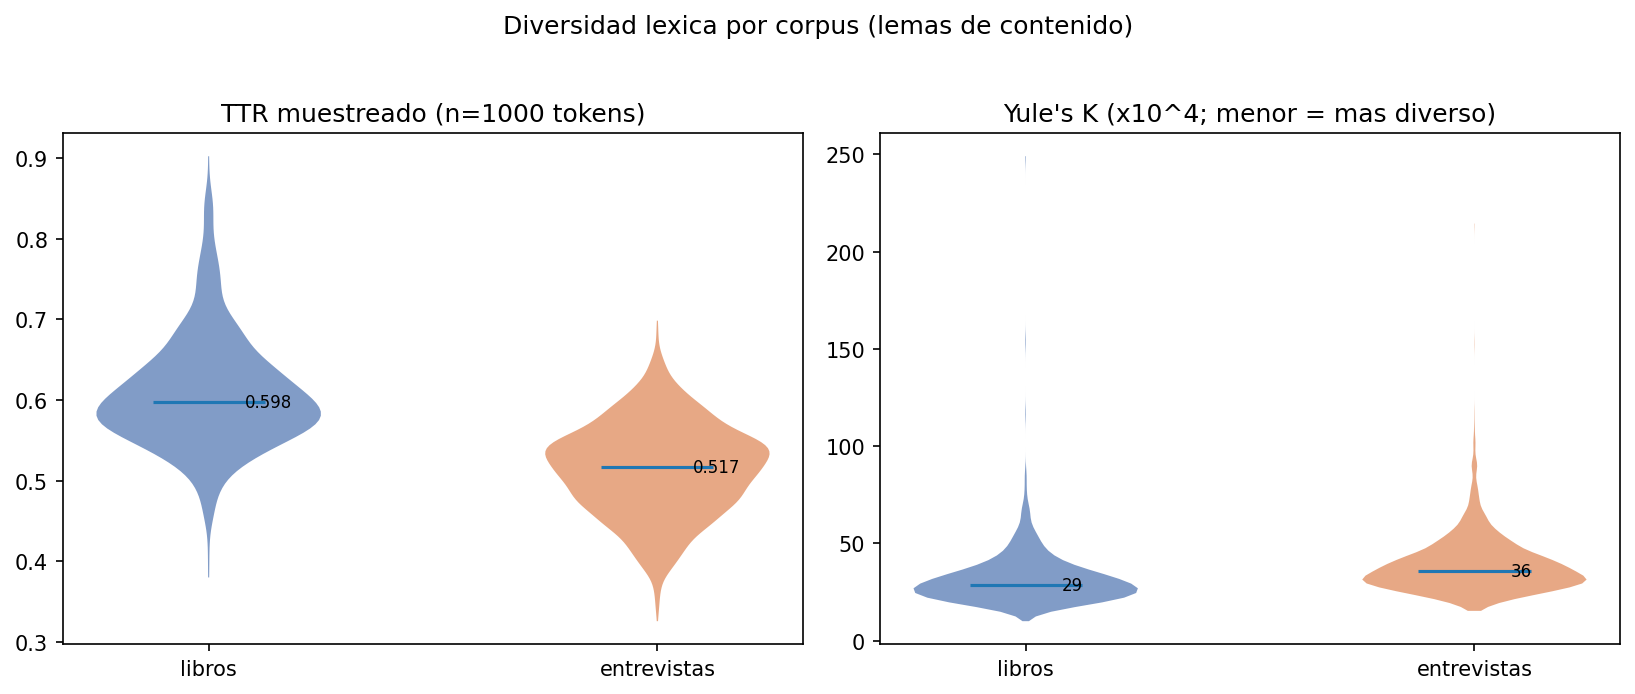
\includegraphics[width=0.60\textwidth]{figuras/eda_diversidad_lexica.png}
    \caption{Diversidad léxica por documento: TTR con muestreo de n=1.000 y Yule K, libros vs. entrevistas. Conclusión: los libros son sistemáticamente más diversos incluso al controlar la longitud; la brecha de registro es una propiedad del corpus y no un artefacto de la asimetría de tamaños, lo que anticipa el desajuste léxico que enfrenta el modelo de IR.}
    \label{fig:diversidad}
\end{figure}

\subsection{Frecuencias, nubes y comparación léxica}

Los vocabularios frecuentes confirman dos mundos léxicos y se analizaron con tres instrumentos complementarios. Primero, las frecuencias: en libros dominan sustantivos institucionales (\textit{armado, víctima, grupo, persona, violencia, comisión, mujer, conflicto}); en entrevistas dominan verbos y formas de narración oral (\textit{gente, llegar, año, pasar, cosa, venir, salir, conocido, persona, querer}). Segundo, las nubes de uni/bi/trigramas construidas desde los top-30 de cada corpus, que ofrecen una lectura visual inmediata y, con bigramas y trigramas, muestran colocaciones que el unigrama oculta. Tercero, el solapamiento de vocabulario, que es bajo: \textbf{Jaccard = 0,221} con 25.851 tipos compartidos, aunque la cobertura de tokens es asimétrica y alta (el vocabulario de libros cubre el 95,7\,\% de los tokens de las entrevistas y el de entrevistas el 98,3\,\% de los de libros). Medir tipos y tokens por separado evita la lectura simplista de que ambos corpus apenas comparten léxico: comparten poco vocabulario, pero ese poco cubre casi todo el texto.

\begin{figure}[htbp]
    \centering
    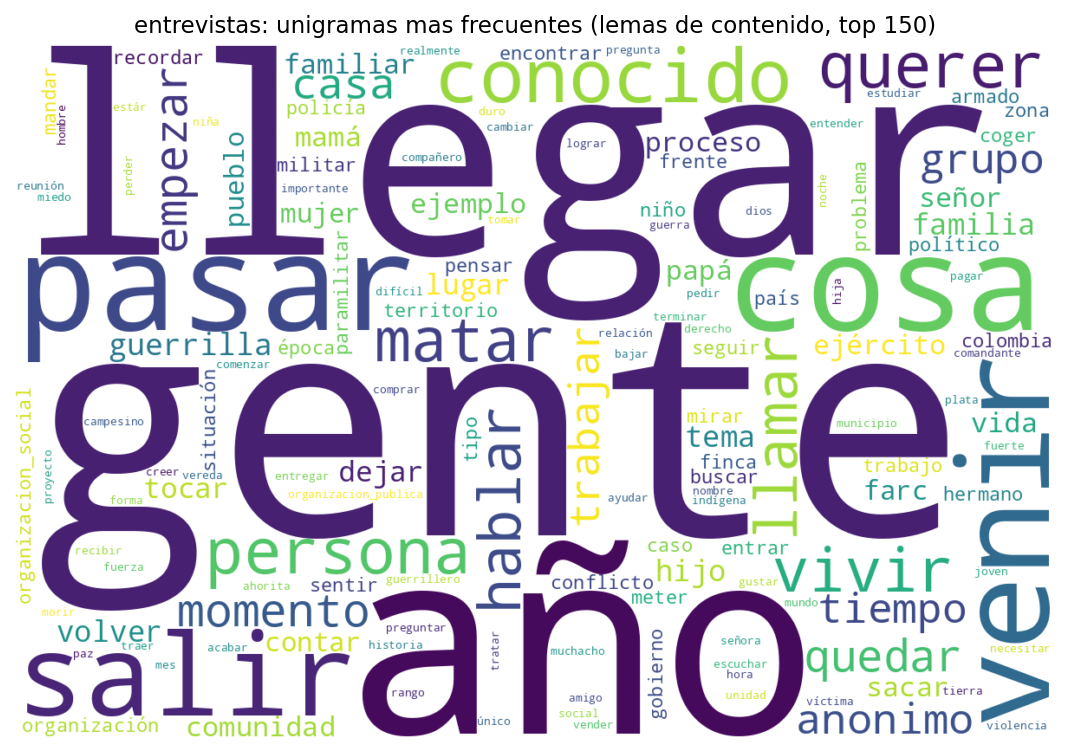
\includegraphics[width=0.52\textwidth]{figuras/eda_entrevistas_nube_unigramas.png}
    \caption{Nube de unigramas de las entrevistas. Predominan verbos de narración y términos genéricos del relato oral. Conclusión: el vocabulario de consulta es funcional pero poco discriminativo por sí mismo, lo que explica que el matching léxico recupere segmentos plausibles aunque a menudo genéricos (Sección~\ref{sec:p3}).}
    \label{fig:nube-entrevistas}
\end{figure}

\begin{figure}[htbp]
    \centering
    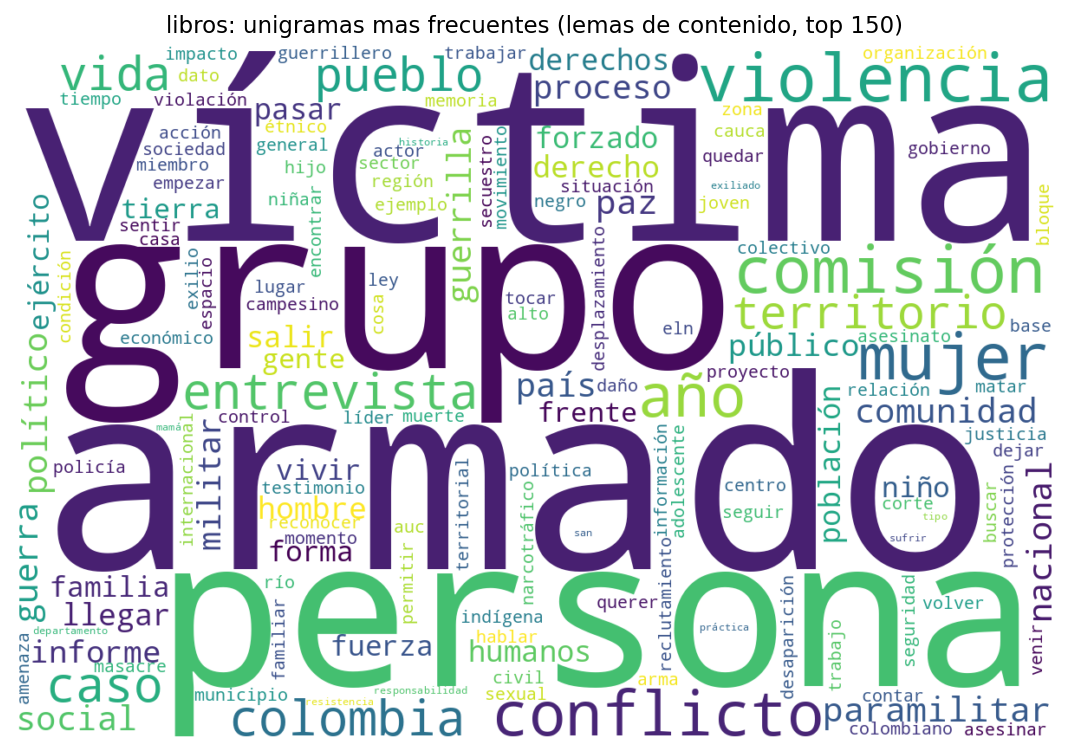
\includegraphics[width=0.52\textwidth]{figuras/eda_libros_nube_unigramas.png}
    \caption{Nube de unigramas de los libros. Predominan sustantivos institucionales y temáticos del conflicto. Conclusión: la intersección de ambos vocabularios es el espacio donde el TF-IDF puede conectar una entrevista con una sección; fuera de esa intersección, ni los términos orales ni los institucionales ayudan al matching.}
    \label{fig:nube-libros}
\end{figure}

La comparación por \textbf{log-odds} con prior informativo (Monroe et al. \cite{monroe2008fightin}) confirma el patrón y se prefirió sobre una prueba de $\chi^2$ por dos razones: las pruebas de independencia se vuelven inestables con términos raros y frecuencias esperadas pequeñas, y no ofrecen una medida con signo e interpretación directa de cuán distintivo es un término. En libros son distintivos términos institucionales y transmedia (\textit{transmedia} 8,0; \textit{externas} 7,8; \textit{microdato} 7,4); en entrevistas lo son las categorías canónicas (\textit{anonimo} 9,1; \textit{organizacion\_social} 8,5; \textit{organizacion\_publica} 8,2), lo que constituye evidencia de que la normalización capturó vocabulario real del habla, y formas orales como \textit{far} (519 ocurrencias, ``las FAR'') frente a \textit{farc} en los libros. Ese desajuste (\textit{far/farc}) es relevante para el IR: una misma entidad se escribe distinto según el registro y el modelo solo puede alinearla si comparte alguna forma. El cruce cualitativo con el tesauro mostró que 14 de los 50 términos distintivos tienen etiqueta SKOS, sin que ello justifique integrarlo al modelo (Sección~\ref{sec:datos}).

\begin{figure}[htbp]
    \centering
    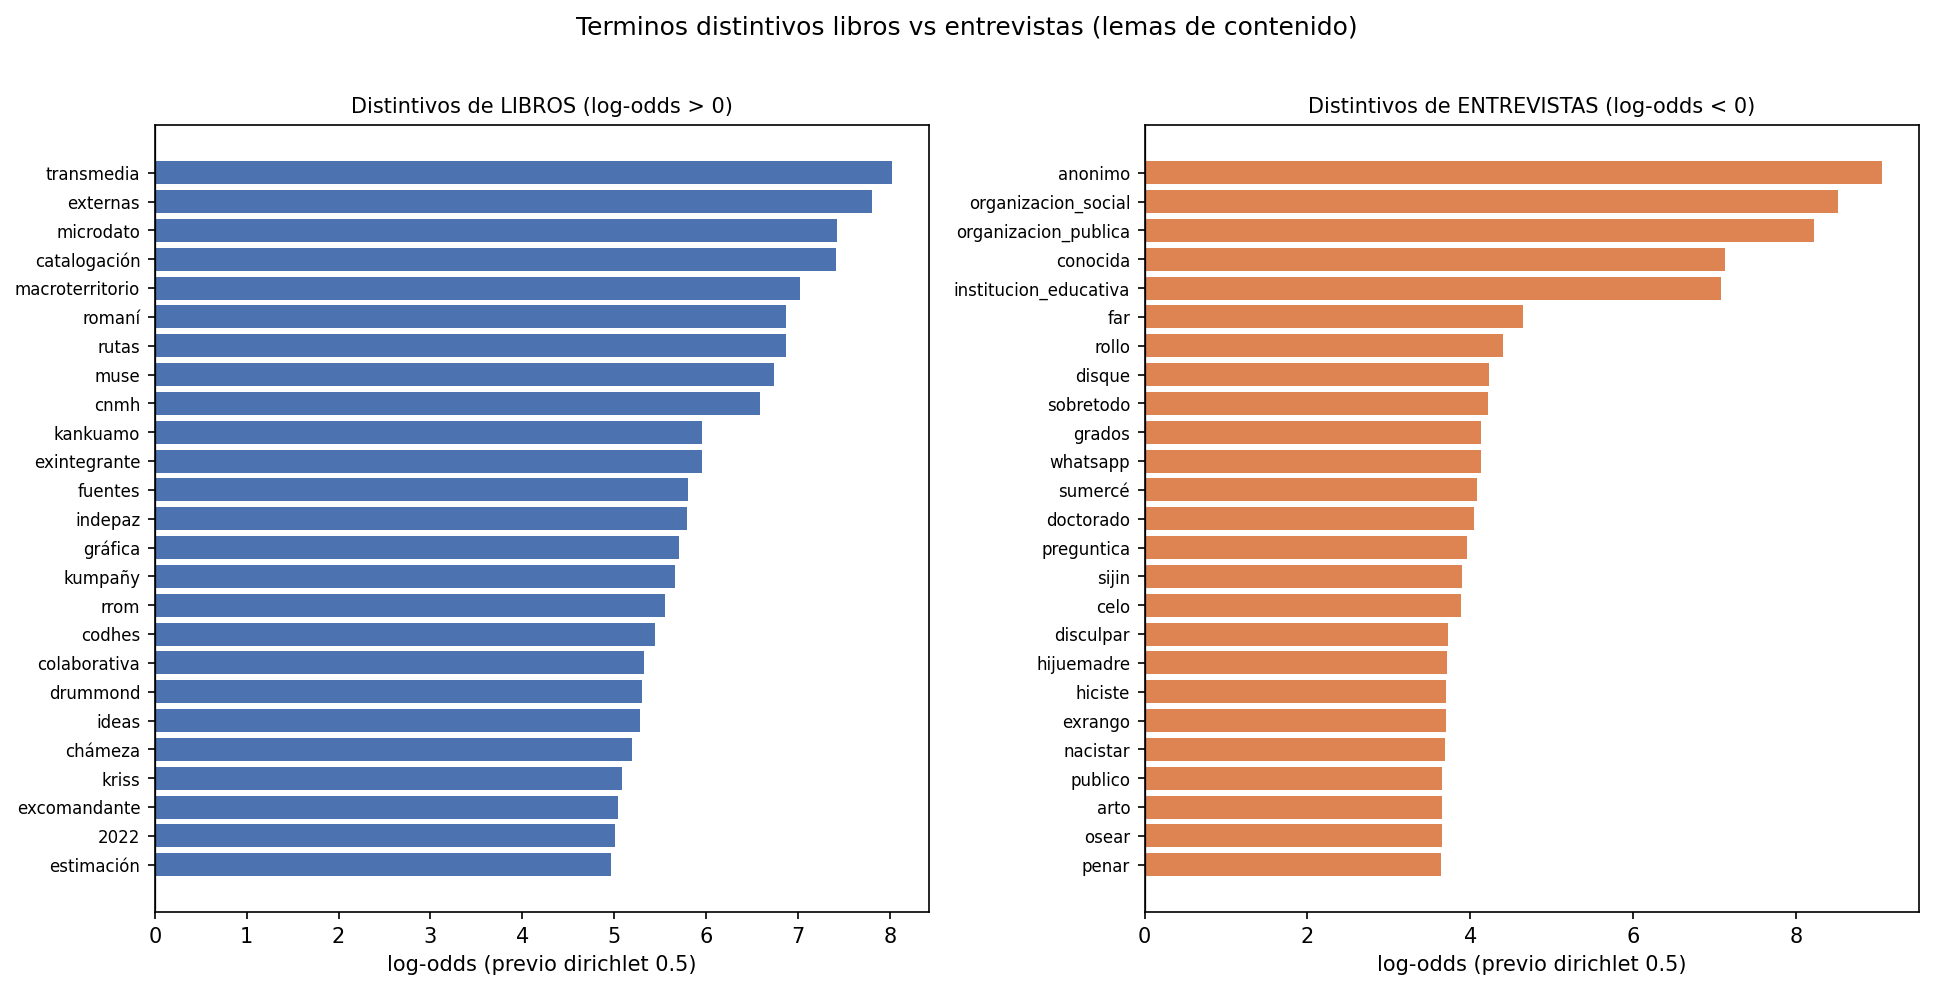
\includegraphics[width=0.70\textwidth]{figuras/eda_comparacion_distintivos_logodds.png}
    \caption{Términos más distintivos de cada corpus según log-odds (top-25 bidireccional). Conclusión: los distintivos de entrevistas son en buena parte categorías canónicas de anonimización, prueba de que la transformación estructural introdujo vocabulario útil; los de libros son institucionales, lo que anticipa que el solape temático fino dependerá de pocos términos compartidos.}
    \label{fig:logodds}
\end{figure}

\subsection{Near-duplicates}

Con Jaccard de \textit{shingles} de 5 lemas se verificaron 368 pares candidatos y se detectaron \textbf{345 pares con similitud $>$0,85}, que involucran 526 documentos únicos en 242 grupos ($\approx$21\,\% de las entrevistas). El procedimiento combina \textit{minhash} (k=60) y LSH (20$\times$3) para generar candidatos, seguido de verificación exacta del Jaccard, siguiendo el esquema de Broder \cite{broder1997resemblance}: la aproximación reduce el costo de comparar todos los pares y la verificación exacta garantiza que el conteo final no dependa de la firma. El umbral 0,85 es deliberadamente alto, de modo que los pares reportados son casi idénticos y no meramente similares. Se conservan por integridad del corpus oficial: entrevistas casi idénticas producen rankings casi idénticos y sobreestiman la cobertura, por lo que se documentan como límite de la evaluación en lugar de eliminarse; la deduplicación queda como mejora futura.

\begin{figure}[htbp]
    \centering
    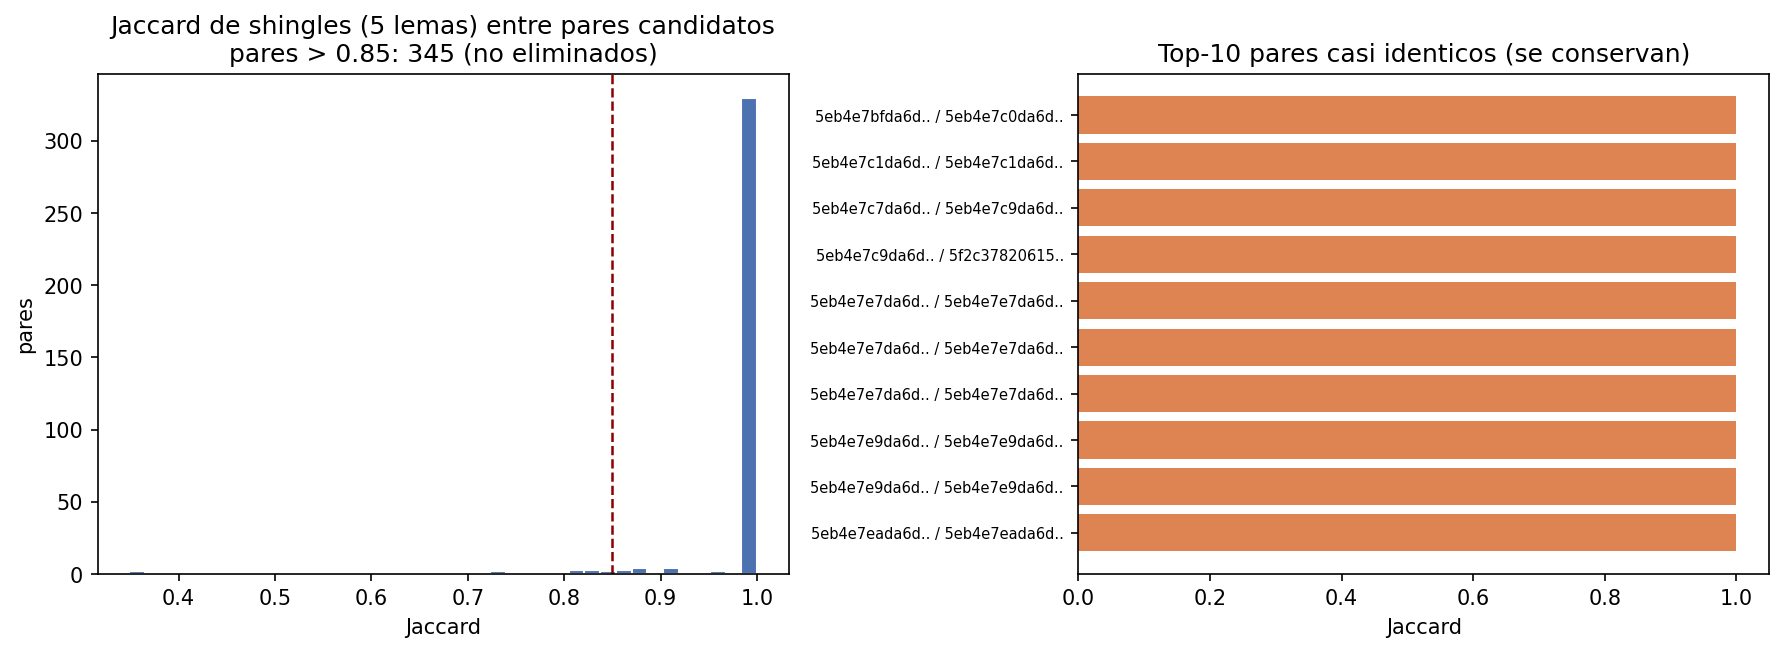
\includegraphics[width=0.55\textwidth]{figuras/eda_near_duplicates_entrevistas.png}
    \caption{Distribución de similitud de los pares candidatos a near-duplicate (shingles de 5 lemas). La masa a la derecha del umbral 0,85 concentra los 345 pares casi idénticos. Conclusión: el corpus contiene duplicación real (a menudo variantes de la misma declaración o reentrevistas) que se documenta como límite de la evaluación, no como error que deba limpiarse.}
    \label{fig:neardups}
\end{figure}

\begin{definicion}[Documentos casi idénticos]
Dos documentos $A$ y $B$ son casi idénticos a nivel de \textit{shingles} de $k$ tokens cuando su similitud de Jaccard $J(A,B)=|S(A)\cap S(B)|\,/\,|S(A)\cup S(B)|$ supera un umbral alto (en este trabajo 0,85), donde $S(\cdot)$ es el conjunto de fragmentos contiguos de $k$ tokens. La medida es independiente del orden global del documento y por eso es robusta a inserciones o reordenamientos locales.
\end{definicion}

\subsection{Decisiones de configuración congeladas en el EDA}

El EDA no solo describe: fija los parámetros del modelo con evidencia. Primero, \texttt{min\_df=2} se justificó con el \textbf{43,2\,\% de hapax} del vocabulario (14.365 de 33.277 tipos con frecuencia documental 1): conservarlos añadiría ruido irrepetible al espacio de términos, pues un tipo que aparece una sola vez no puede discriminar entre documentos. Segundo, \texttt{max\_df=0,85} se justificó porque \textbf{solo 6 tipos} aparecen en más del 85\,\% de los segmentos: el umbral descarta términos omnipresentes sin recortar vocabulario temático. Tercero, \texttt{ngram\_range=(1,2)} busca colocaciones de dominio (\textit{desaparición forzada}, \textit{violencia sexual}, \textit{falsos positivos}) que los unigramas pierden; el experimento comparativo posterior (Sección~\ref{sec:p3}) cuantificó su aporte. Cuarto, \texttt{sublinear\_tf=True} y \texttt{norm='l2'} siguen la formulación clásica de Salton y Buckley \cite{salton1988term} y Manning et al. \cite{manning2008introduction}. Estas decisiones se congelaron en \texttt{config/tfidf\_config.json} y viajan embebidas en el notebook, de modo que la configuración del experimento es reproducible sin depender de archivos externos.


\section{P3 --- Modelo de IR con TF-IDF}\label{sec:p3}

\subsection{Dirección del matching y representación}

La dirección del matching quedó fija: \textbf{cada entrevista es una query y la colección son los 917 segmentos de libro}. La alternativa transpuesta se descartó porque el entregable del taller pide, para cada entrevista, las secciones del Informe afines; además, la colección debe ser estable y de tamaño moderado ---condición que cumplen los segmentos y no las 2.486 transcripciones---, y la dirección inversa habría duplicado el trabajo con una estabilidad menor. La representación es TF-IDF con saturación sublineal y normalización l2 \cite{salton1988term,manning2008introduction}, implementada con \texttt{TfidfVectorizer} de scikit-learn \cite{scikit2024tfidf} sobre los textos lematizados; se prefirió la implementación de la biblioteca, ya validada y reproducible, antes que una versión propia, porque el objetivo del punto 3 es el modelo de IR y no la aritmética de la vectorización (la implementación manual se reserva para BM25 y Rocchio, como exige el punto 4):

\begin{equation}\label{eq:tfidf}
\widetilde{tf}(t,d) = 1+\ln tf(t,d), \qquad
idf(t) = \ln\!\left(\frac{1+N}{1+df(t)}\right)+1, \qquad
w(t,d) = \widetilde{tf}(t,d)\cdot idf(t),
\end{equation}

\noindent donde $tf(t,d)$ es la frecuencia del término $t$ en el documento $d$, $df(t)$ su frecuencia documental y $N$ el número de documentos de la colección. Cada documento se normaliza a norma unitaria:

\begin{equation}\label{eq:vector}
v_d = \frac{w(d)}{\lVert w(d)\rVert_2}.
\end{equation}

\noindent La relevancia entre la consulta $q$ (entrevista) y el documento $d$ (segmento) se mide por similitud coseno:

\begin{equation}\label{eq:coseno}
sim(q,d) = \cos(\theta_{q,d}) = \frac{v_q\cdot v_d}{\lVert v_q\rVert_2\,\lVert v_d\rVert_2} = v_q\cdot v_d,
\end{equation}

\noindent igualdad final válida porque ambos vectores están normalizados. El \textit{fit} del vectorizador se hace \textbf{solo sobre la colección} y las consultas se transforman con el mismo vectorizador: no hay fuga de información de las entrevistas hacia el vocabulario ni hacia los pesos IDF, porque las consultas son datos de entrada que no deben influir en la definición del espacio de representación.

\begin{definicion}[Similitud coseno]
Dados dos vectores no nulos $v_q, v_d \in \mathbb{R}^{F}$, la similitud coseno es el coseno del ángulo que forman, $\cos(\theta)=v_q\cdot v_d\,/\,(\lVert v_q\rVert_2\lVert v_d\rVert_2)\in[-1,1]$. Es invariante a la escala de los vectores y, en IR, mide la orientación temática compartida con independencia de la longitud de los documentos.
\end{definicion}

\subsection{Configuración y resultado del ranking}

La configuración congelada (Tabla~\ref{tab:config-tfidf}) produjo un vocabulario de \textbf{118.748 features} (18.864 unigramas y 99.884 bigramas) con densidad de 0,0082, valor coherente con una matriz dispersa típica de IR. La puntuación por lotes tardó 10,0 s (semilla 42) y generó \texttt{ranking\_top5.csv} y \texttt{ranking\_top10.csv} (12.420 filas el primero). El modelo recupera al menos un segmento para \textbf{2.484 de 2.486 entrevistas (cobertura 99,92\,\%)}; las 2 restantes son los documentos vacíos legítimos ya documentados. El score top-1 tiene media 0,1468, mediana 0,138 y rango 0,070-0,572. La semilla fija y la ejecución por lotes hacen que el ranking sea determinista, condición necesaria para que las comparaciones entre variantes (Sección~\ref{sec:p3}) y entre métodos (Sección~\ref{sec:p4}) sean atribuibles a los cambios introducidos y no al azar.

\begin{table}[htbp]
    \centering
    \caption{Parámetros del modelo TF-IDF y su justificación empírica (datos del EDA).}
    \small
    \setlength{\tabcolsep}{5pt}
    \begin{tabular}{l l p{7.1cm}}
    \toprule
    Parámetro & Valor & Justificación \\
    \midrule
    \texttt{ngram\_range} & (1,2) & colocaciones de dominio que los unigramas pierden \\
    \texttt{min\_df} & 2 & 43,2\,\% de hapax (14.365/33.277 tipos con df=1) \\
    \texttt{max\_df} & 0,85 & solo 6 tipos superan el 85\,\% de los segmentos \\
    \texttt{sublinear\_tf} & True & saturación del tf (Salton y Buckley, 1988) \\
    \texttt{norm} & l2 & coseno estable (Manning et al., 2008) \\
    \texttt{use\_idf}/\texttt{smooth\_idf} & True/True & IDF suavizado de scikit-learn \\
    \bottomrule
    \end{tabular}
    \label{tab:config-tfidf}
\end{table}

La distribución del top-1 por tomo revela un sesgo marcado: \textbf{76,77\,\% en TESTIMONIAL} (1.907 entrevistas), seguido de FUERA 5,19\,\%, NARRATIVA 4,35\,\%, ETNICO 3,82\,\% y VIOLACIONES 2,94\,\%. La revisión del fenómeno lo interpretó como \textbf{efecto de dominio, no artefacto}: el tomo testimonial reproduce el registro oral de las víctimas \cite{castillejo2023escuchar} y, por tanto, comparte vocabulario funcional con las consultas. Para sostener esa lectura se descartaron explicaciones alternativas: ni la longitud de las queries ni las categorías canónicas explican la magnitud del efecto, y el modelo base se regeneró idéntico en 2.484/2.484 top-1, lo que descarta un artefacto de ejecución. El sesgo es, entonces, una propiedad del corpus que debe declararse y medirse (Secciones~\ref{sec:p4} y~\ref{sec:p5}), no un error que se oculte.

\subsection{Evaluación cualitativa}

Sin gold estándar, la evaluación se hizo sobre una \textbf{muestra determinista (semilla 42), estratificada por tomo, de 30 pares (entrevista, segmento top-1)} con el top-3 completo, etiquetados por el equipo en tres clases \{relacionado, parcial, no\}. La estratificación garantiza que todos los tomos estén representados aunque TESTIMONIAL domine el ranking; las tres clases permiten distinguir el acierto específico del solape genérico, y el top-3 completo permite observar si el resultado relevante quedó cerca del primer puesto. La Tabla~\ref{tab:evaluacion} resume los resultados: 16 pares ``relacionado'', 14 ``parcial'' y \textbf{0 ``no''}. El matching léxico es funcional pero impreciso: con criterio estricto P@1 = 0,5333 y P@3 = 0,7667; con criterio aceptable (``relacionado''+``parcial'') ambos llegan a 1,0, porque todo el corpus versa sobre el conflicto y cualquier entrevista de víctima solapa mínimamente con casi cualquier segmento. El hallazgo fino es que en \textbf{7 de 30 consultas (23\,\%)} el top-1 es ``parcial'' y el match ``relacionado'' está en las posiciones 2-3: el primer resultado no siempre es el más específico. Hay aciertos nítidos cuando el léxico es específico (amenaza de masacre $\rightarrow$ \texttt{HALLAZGOS-p129-las-masacres}, 0,132) y fallos por solape genérico en testimonios (excombatiente indígena amazónica $\rightarrow$ \texttt{TESTIMONIAL-p401-senderos-pedregosos}). La decisión de iteración fue \textbf{no crear un experimento 2}: el criterio del plan (P@1 aceptable $\geq$ 0,6) ya se cumple con 1,0 y el problema diagnosticado no es el registro oral ---las muletillas ya están en parada--- sino la falta de discriminación temática fina, que este tipo de evaluación sobre 30 pares tampoco puede resolver sin un gold externo. Los límites de la muestra (tamaño reducido, etiquetado por el propio equipo y sin acuerdo inter-etiquetador) se declaran en la Sección~\ref{sec:p6}.

\begin{table}[htbp]
    \centering
    \caption{Evaluación cualitativa sobre 30 pares (entrevista, top-1 con top-3 completo), semilla 42. Fuente: \texttt{resultados/evaluacion\_metricas.json}.}
    \small
    \setlength{\tabcolsep}{6pt}
    \begin{tabular}{l r}
    \toprule
    Métrica & Valor \\
    \midrule
    Etiquetas relacionado / parcial / no & 16 / 14 / 0 \\
    P@1 estricto (solo ``relacionado'') & 0,5333 \\
    P@1 aceptable (``relacionado''+``parcial'') & \textbf{1,0000} \\
    P@3 (al menos un ``relacionado'' en r1-r3) & 0,7667 \\
    P@3 aceptable (``relacionado''+``parcial'' en r1-r3) & \textbf{1,0000} \\
    Top-1 ``parcial'' con match ``relacionado'' en r2-r3 & 7 de 30 (23\,\%) \\
    \bottomrule
    \end{tabular}
    \label{tab:evaluacion}
\end{table}

\subsection{Variantes del modelo}

Para medir la contribución de cada decisión de preprocesado se compararon tres variantes contra el base, cada una aislando un factor: (A) solo unigramas (\texttt{ngram\_range=(1,1)}), que mide el aporte de los bigramas; (B) sin la parada de muletillas, que mide el efecto de las 51 muletillas del habla; y (C) sin las 62 correcciones de lemas, que mide el efecto del ajuste morfológico. La Tabla~\ref{tab:variantes} reporta la coincidencia del top-1 con el modelo base. La lectura es directa: los \textbf{bigramas aportan la mayor parte del cambio} (sin ellos el top-1 solo coincide en 54,8\,\%), las muletillas mueven poco (84,6\,\% de coincidencia) y las correcciones muy poco (96,6\,\%). La configuración base es, además, la más estable de las cuatro. Que las correcciones de lemas muevan tan poco el ranking no invalida su inclusión: su efecto es de calidad lingüística en casos puntuales y su costo es despreciable, mientras que la ganancia de los bigramas justifica el aumento de dimensionalidad del vocabulario.

\begin{table}[htbp]
    \centering
    \caption{Variantes del modelo base y coincidencia del top-1 con el base (2.484 queries). Fuente: \texttt{resultados/ranking\_top5\_\{A,B,C\}.csv}.}
    \small
    \setlength{\tabcolsep}{6pt}
    \begin{tabular}{l r r}
    \toprule
    Variante & Cambio respecto al base & Coincidencia top-1 \\
    \midrule
    A --- sin bigramas (ngram 1,1) & 45,2\,\% & 54,8\,\% \\
    B --- sin parada de muletillas & 15,4\,\% & 84,6\,\% \\
    C --- sin correcciones de lemas & 3,4\,\% & 96,6\,\% \\
    \bottomrule
    \end{tabular}
    \label{tab:variantes}
\end{table}


\section{P4 --- Métricas de relevancia implementadas manualmente}\label{sec:p4}

El punto 4 exige implementar \textbf{manualmente} Rocchio y Okapi BM25. Ambas se programaron desde cero en la sección 03b del notebook (sin \texttt{rank\_bm25} ni librerías de retroalimentación) sobre la misma dirección de matching, el mismo vocabulario y las mismas matrices del modelo base: la única diferencia es la función de puntuación, de modo que las diferencias de ranking sean atribuibles al modelo de relevancia y no a cambios en la representación. Se implementaron desde cero, además de por exigencia del enunciado, para poder verificar cada componente contra cálculos hechos a mano. Como utilidad de tokenización y conteo se usó \texttt{CountVectorizer}, práctica admitida por el enunciado.

\subsection{Okapi BM25}

La fórmula implementada (Robertson y Walker \cite{robertson1994simple}; véase también Robertson y Zaragoza \cite{robertson2009probabilistic}) es:

\begin{equation}\label{eq:bm25}
score(q,d) = \sum_{t\in q} qtf(t)\cdot IDF(t)\cdot
\frac{tf(t,d)\,(k_1+1)}{tf(t,d)+k_1\!\left(1-b+b\,\dfrac{|d|}{avgdl}\right)},
\end{equation}

\begin{equation}\label{eq:bm25idf}
IDF(t) = \ln\!\left(\frac{N-df(t)+0{,}5}{df(t)+0{,}5}+1\right),
\end{equation}

\noindent con $qtf(t)$ la frecuencia del término en la consulta, $tf(t,d)$ su frecuencia cruda en el documento, $|d|$ la longitud del documento y $avgdl$ la longitud media de la colección. Los parámetros se fijaron en los valores por defecto habituales de la literatura para colecciones de documentos de longitud media (rangos típicos $k_1\in[1{,}2;\,2{,}0]$ y $b\approx 0{,}75$): $k_1=1{,}5$ controla la saturación (el denominador tiende a $k_1+1$, de modo que las repeticiones dejan de aportar marginalmente) y $b=0{,}75$ controla la normalización por longitud, de forma que un segmento extenso no acumule score solo por tamaño. Se prefirieron estos valores antes que una búsqueda de hiperparámetros porque no existe gold estándar con el cual optimizarlos, y ajustarlos contra el ranking del modelo base habría sesgado la comparación; el ajuste fino queda como mejora futura. El IDF de Robertson-Sparck Jones premia términos raros y queda siempre positivo con el suavizado $+0{,}5$; con 43,2\,\% de hapax en el vocabulario, este componente reordena la cola de términos respecto del IDF suavizado de scikit-learn.

Sobre la colección de 917 segmentos por 118.748 términos (891.794 entradas no nulas) resultó $avgdl=\mathbf{1.466{,}26}$ términos del vocabulario, con longitudes entre 155 y 2.741. Es importante precisar la \textbf{unidad de $|d|$}: se mide en términos del vocabulario (unigramas y bigramas, cada bigrama cuenta como un término adicional), no en lemas de contenido (1.007,5 de media: 923.912/917 tras la parada del IR). Es la longitud que exige Okapi sobre el mismo espacio de términos que ``ve'' el TF-IDF; reportarla en lemas habría hecho incomparable el denominador con la frecuencia de término usada por la fórmula. El auto-check con tres documentos calculados a mano dio esperado $[0{,}671434,\ 0{,}552945,\ 0{,}0]$ = obtenido (tolerancia $10^{-12}$), evidencia de que la implementación reproduce la fórmula y no solo de que produce números plausibles. El ranking BM25 (12.420 filas) concentra el top-1 en TESTIMONIAL con 1.863 entrevistas (\textbf{75,0\,\%}) y coincide con el top-1 del base en el \textbf{57,0\,\%} de las 2.484 consultas comunes (umbral de cordura $>$40\,\%).

\subsection{Rocchio con pseudo-relevancia}

El clasificador de Rocchio \cite{rocchio1971relevance} expande la consulta hacia el centroide de los documentos relevantes y la aleja del de los no relevantes:

\begin{equation}\label{eq:rocchio}
q' = \alpha\, q + \frac{\beta}{|D_r|}\sum_{d\in D_r} d \;-\; \frac{\gamma}{|D_{nr}|}\sum_{d\in D_{nr}} d,
\qquad \alpha=1{,}0,\quad \beta=0{,}75,\quad \gamma=0{,}15,
\end{equation}

\noindent donde $q$ es la consulta del base, $D_r$ el conjunto de documentos relevantes y $D_{nr}$ el de no relevantes. $\alpha$ ancla la consulta original, $\beta$ la expande hacia los relevantes y $\gamma$ resta los no relevantes. Los valores elegidos son conservadores y responden a que los juicios de relevancia no son confiables: $\alpha=1$ mantiene intacta la consulta original, $\beta=0{,}75<\alpha$ deja que la expansión influya sin dominarla y $\gamma=0{,}15$ resta poco porque los negativos por pseudo-relevancia son ruidosos al no estar etiquetados. Como no hay gold, se usa \textbf{retroalimentación por pseudo-relevancia} \cite{manning2008introduction}: el top-5 del ranking base actúa como $D_r$ y el bottom-5 (los peores scores) como $D_{nr}$, una elección estándar cuando no hay juicios humanos y que supone que los extremos del ranking contienen la señal más aprovechable. La implementación \textbf{conserva los pesos negativos sin truncarlos (clamp) a cero}, porque el término de $D_{nr}$ debe restar de verdad; el auto-check con vectores conocidos lo verifica: la expansión manual $[1{,}375,\ 0{,}375,\ -0{,}15]$ coincide con la implementada tras normalizar l2, $[0{,}959464,\ 0{,}261672,\ -0{,}104669]$, con el término de $\beta$ positivo y el de $\gamma$ negativo.

El re-rankeo afectó a 2.484 consultas y cambió el top-1 en \textbf{743 (29,9\,\%)}; el nuevo top-1 se concentró aún más en TESTIMONIAL: \textbf{1.947 entrevistas (78,4\,\%)}. Como control de sensibilidad se añadió la variante $k=3$ ($D_r$ = top-3, $D_{nr}$ = bottom-3), que responde a cuánto depende el resultado del tamaño del feedback: el top-1 cambió en \textbf{596 de 2.484 consultas (24,0\,\%)} respecto del base y en \textbf{563 (22,7\,\%)} respecto de $k=5$. Es decir, $k=5$ es la configuración más agresiva (su centroide incorpora más vocabulario del tomo dominante) mientras $k=3$ se mantiene más cerca del ranking base (TESTIMONIAL pasa de 1.947 a 1.933 top-1). La dirección del efecto no cambia, pero su magnitud sí: \textbf{cualquier uso de Rocchio debe reportar $k$}, y $k=5$ se conserva como configuración principal por corresponder al diseño original de la comparación.

\subsection{Comparación entre métricas y discusión}

Sin gold, la comparación es de \textbf{acuerdo}: se mide el solapamiento de \textbf{conjunto} del top-$k$ (qué fracción de ítems comparten, con independencia del orden) y la coincidencia de \textbf{posición} exacta (Tabla~\ref{tab:acuerdo}), dos métricas que juntas distinguen compartir inventario de compartir orden. De las 2.484 consultas comparables, \textbf{1.112 coinciden en el top-1 de los tres métodos y 296 difieren en los tres}.

\begin{table}[htbp]
    \centering
    \caption{Acuerdo entre métodos sobre 2.484 consultas. ``Conjunto top-1/top-5'' = fracción de elementos compartidos del conjunto; ``posición 5'' = identidad del ítem en la posición 5. Fuente: sección 03b del notebook.}
    \small
    \setlength{\tabcolsep}{6pt}
    \begin{tabular}{l r r r}
    \toprule
    Par de métodos & Top-1 conjunto & Posición 5 & Conjunto top-5 \\
    \midrule
    TF-IDF base vs. BM25 & 57,0\,\% & 11,8\,\% & 65,7\,\% \\
    TF-IDF base vs. Rocchio & 70,1\,\% & 48,8\,\% & \textbf{100,0\,\%} \\
    BM25 vs. Rocchio & 50,6\,\% & 10,5\,\% & 65,7\,\% \\
    \bottomrule
    \end{tabular}
    \label{tab:acuerdo}
\end{table}

\begin{table}[htbp]
    \centering
    \caption{Top-1 por tomo para los tres métodos (cada columna suma 2.484 consultas con match). Fuente: \texttt{resultados/ranking\_bm25.csv}, \texttt{ranking\_rocchio.csv} e \texttt{ir\_tfidf\_report.json}.}
    \small
    \setlength{\tabcolsep}{6pt}
    \begin{tabular}{l r r r}
    \toprule
    Tomo & TF-IDF base & BM25 & Rocchio \\
    \midrule
    TESTIMONIAL & 1.907 (76,77\,\%) & 1.863 (75,0\,\%) & \textbf{1.947} (78,4\,\%) \\
    FUERA & 129 & 127 & 123 \\
    NARRATIVA & 108 & 103 & 84 \\
    ETNICO & 95 & 115 & 99 \\
    VIOLACIONES & 73 & 105 & 71 \\
    HALLAZGOS & 53 & 43 & 59 \\
    CUERPO & 50 & 52 & 38 \\
    SUFRIR & 46 & 55 & 45 \\
    NNA & 22 & 19 & 17 \\
    CONVOCATORIA & 1 & 2 & 1 \\
    \bottomrule
    \end{tabular}
    \label{tab:top1-tomo}
\end{table}

Cuatro lecturas se desprenden de las tablas. Primero, \textbf{BM25 y TF-IDF comparten señal pero ordenan distinto}: el 57,0\,\% de top-1 idéntico y el 65,7\,\% de conjunto top-5 indican señal común, pero solo el 11,8\,\% coincide en la posición 5 exacta, porque BM25 normaliza por longitud ($b=0{,}75$, sin ventaja por volumen) y usa un IDF más agresivo con los términos raros que el \texttt{smooth\_idf} de scikit-learn. Segundo, \textbf{Rocchio re-rankea, no sustituye el inventario}: conserva el 70,1\,\% de los top-1 y su conjunto top-5 es \textbf{idéntico al del base en el 100,0\,\%} (posición 5 exacta en 48,8\,\%), lo que muestra que domina $\beta$ y que los bottom-5 casi siempre puntúan 0, con lo que $\gamma$ aporta poco; además hereda el sesgo del base (desplazamiento de consulta o \textit{query drift}). Tercero, \textbf{el sesgo TESTIMONIAL es del dominio, no de la función}: los tres métodos concentran el top-1 en el mismo tomo (76,77\,\% / 75,0\,\% / 78,4\,\%). Cuarto, el acuerdo mide \textbf{consistencia, no acierto}: sin gold no hay P@$k$ real para BM25 y Rocchio, y la única verificación humana es la muestra etiquetada de la Sección~\ref{sec:p3}; por eso el acuerdo se interpreta como evidencia de estabilidad del ranking, no de relevancia. Cualitativamente, donde los tres coinciden hay solape específico; donde difieren, el base devuelve un testimonial genérico, BM25 premia términos raros y Rocchio reordena hacia el centroide (para una misma entrevista: \textit{Algo me atravesó} vs. \textit{¿Escuchaste eso?} vs. \textit{Lo inhabitable}).

\begin{lstlisting}[language=Python,caption={Funciones propias de BM25 y Rocchio (signaturas; el código completo está en \texttt{notebooks/}\texttt{Taller\_4\_IR\_CEV.ipynb}, sección 03b, y en el repositorio del taller).},label={lst:funciones}]
# --- Okapi BM25 manual (sin librerias de ranking) ---
construir_matriz_tf(docs_lemas, ngram_range=(1,2), min_df=2, max_df=0.85)
calcular_longitudes_y_df(matriz_tf)          # |d|, avgdl y df(t)
idf_bm25(df, n_docs)                         # ln((N-df+0.5)/(df+0.5)+1)
puntuar_bm25(query_tf, matriz_tf, idf, longitudes, avgdl, k1=1.5, b=0.75)
rankear_bm25(queries_lemas, docs_lemas, docs_queries, docs_coleccion,
             top_k=5, k1=1.5, b=0.75)

# --- Rocchio manual con pseudo-relevancia ---
rocchio_expandir(q_vec, docs_relevantes, docs_no_relevantes,
                 alpha=1.0, beta=0.75, gamma=0.15)
rankear_rocchio(similitudes_base, x_queries, x_coleccion,
                docs_queries, docs_coleccion, top_k=5,
                n_relevantes=5, n_no_relevantes=5,
                alpha=1.0, beta=0.75, gamma=0.15)
\end{lstlisting}


\section{P5 --- Comparación de corpus: heatmaps y cuadro de vínculos}\label{sec:p5}

\subsection{Heatmap agregado 10$\times$10}

El primer heatmap responde a una pregunta global: \textit{¿los grupos de entrevistas asignados a cada tomo se parecen, en promedio, a ese tomo?} Las filas agrupan las 2.486 entrevistas por el tomo de su top-1 \textbf{BM25}; las columnas son los 10 tomos; la celda $(g,T)$ es la \textbf{similitud coseno TF-IDF media} entre las entrevistas del grupo $g$ y los segmentos del tomo $T$, calculada sobre la matriz del modelo base sin reentrenar nada, de modo que el heatmap mide la organización implícita del corpus y no reajusta el espacio de representación. Se usa la media por par (medida intensiva de afinidad) y no una masa total, de modo que el distinto número de segmentos por tomo no sesga la comparación; el CSV conserva \texttt{n\_entrevistas} por grupo. La diagonal mide la \textbf{coherencia} entre la asignación BM25 y la similitud TF-IDF: si la asignación no fuera más que ruido, la diagonal no debería destacar.

\begin{figure}[htbp]
    \centering
    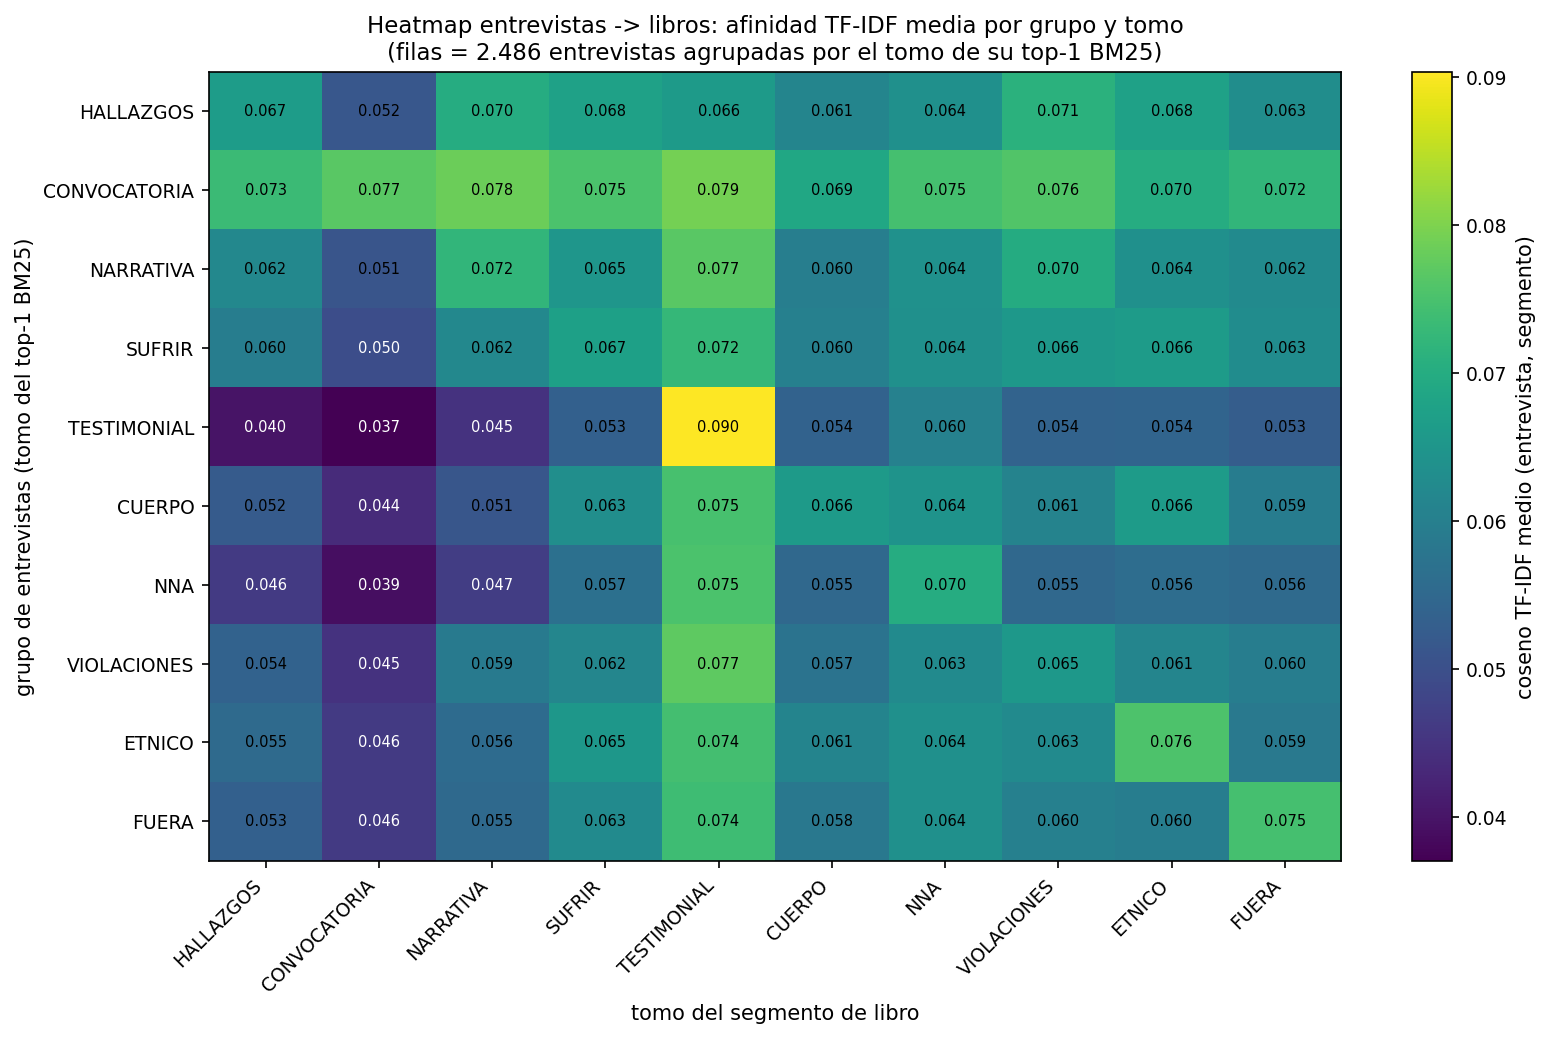
\includegraphics[width=0.60\textwidth]{figuras/heatmap_entrevistas_libros.png}
    \caption{Heatmap agregado 10$\times$10: filas = grupo de entrevistas por tomo del top-1 BM25; columnas = tomo de libro; celda = coseno TF-IDF medio. Conclusión: la diagonal media (0,0725) supera a la afinidad fuera de la diagonal (0,0608) y a la media de fila en 10/10 grupos, de modo que la asignación BM25 captura señal real; sin embargo, el máximo de fila cae fuera de la diagonal en 7/10 grupos (casi siempre en TESTIMONIAL), evidencia visual del sesgo de registro oral.}
    \label{fig:heatmap-agregado}
\end{figure}

\begin{table}[htbp]
    \centering
    \caption{Resumen del heatmap por grupo (coseno TF-IDF medio). ``Máximo de fila'' indica el tomo con mayor afinidad media. Fuente: \texttt{resultados/heatmap\_tomos.csv}.}
    \footnotesize
    \setlength{\tabcolsep}{5pt}
    \begin{tabular}{l r r l c}
    \toprule
    Grupo (n) & Diagonal & Media fila & Máximo de fila & Diag. $>$ media \\
    \midrule
    HALLAZGOS (43) & 0,0666 & 0,0649 & VIOLACIONES 0,0711 & Sí \\
    CONVOCATORIA (2) & 0,0767 & 0,0745 & TESTIMONIAL 0,0793 & Sí \\
    NARRATIVA (103) & 0,0722 & 0,0647 & TESTIMONIAL 0,0766 & Sí \\
    SUFRIR (55) & 0,0674 & 0,0630 & TESTIMONIAL 0,0725 & Sí \\
    TESTIMONIAL (1.863) & \textbf{0,0904} & 0,0540 & TESTIMONIAL 0,0904 & Sí \\
    CUERPO (52) & 0,0662 & 0,0603 & TESTIMONIAL 0,0749 & Sí \\
    NNA (19) & 0,0702 & 0,0556 & TESTIMONIAL 0,0753 & Sí \\
    VIOLACIONES (105) & 0,0655 & 0,0602 & TESTIMONIAL 0,0771 & Sí \\
    ETNICO (115) & 0,0756 & 0,0619 & ETNICO 0,0756 & Sí \\
    FUERA (127) & 0,0747 & 0,0608 & FUERA 0,0747 & Sí \\
    \midrule
    \textbf{Global} & \textbf{0,0725} & --- & --- & \textbf{10/10} \\
    \bottomrule
    \end{tabular}
    \label{tab:heatmap}
\end{table}

La lectura de la Tabla~\ref{tab:heatmap} es matizada. La diagonal media (0,0725) supera a la media fuera de la diagonal (0,0608) y a la media de fila en los 10 grupos: \textbf{la asignación BM25 no es ruido}. TESTIMONIAL concentra 1.863 entrevistas (74,9\,\%) y tiene la diagonal más alta (0,0904), pero su media de fila es la más baja (0,0540), señal de que su afinidad es específica con su propio tomo. El máximo de fila cae en la diagonal solo en 3/10 grupos (TESTIMONIAL, ETNICO, FUERA); en 6 de los 7 restantes cae en TESTIMONIAL y en HALLAZGOS cae en VIOLACIONES (0,0711 vs. 0,0666), lo que constituye una lectura visual del sesgo de registro oral. Fuera de la diagonal dominan TESTIMONIAL (0,066-0,079) y NARRATIVA (0,045-0,078); las celdas más bajas están en CONVOCATORIA. Dos limitaciones deben declararse: CONVOCATORIA tiene n=2 (su diagonal, 0,0767, es frágil) y la agrupación hereda el sesgo TESTIMONIAL, de modo que el heatmap mide coherencia, no corrección.

\subsection{Heatmap top-25 por documento}

El segundo heatmap responde a otra pregunta: \textit{¿qué entrevistas concretas saturan cada eje temático?} Sobre la matriz BM25 completa (2.486$\times$917) se seleccionaron las 25 entrevistas con mayor suma de sus máximos BM25 por tomo; la celda es el \textbf{máximo BM25} de esa entrevista contra cualquier segmento del tomo (no la media). Se eligió el máximo porque el objetivo es identificar vínculos fuertes individuales, que un promedio por grupo disolvería; y se eligieron 25 filas para mantener el gráfico legible conservando los casos más intensos. El máximo de la matriz (32.700,223) coincide con el mejor vínculo BM25 del tomo TESTIMONIAL (Tabla~\ref{tab:vinculos}). Los dos heatmaps se complementan: el agregado resume la visión global y valida la asignación BM25 $\rightarrow$ tomo; el top-25 conserva la \textbf{intensidad individual}, información que el promedio por grupo disuelve.

\begin{figure}[htbp]
    \centering
    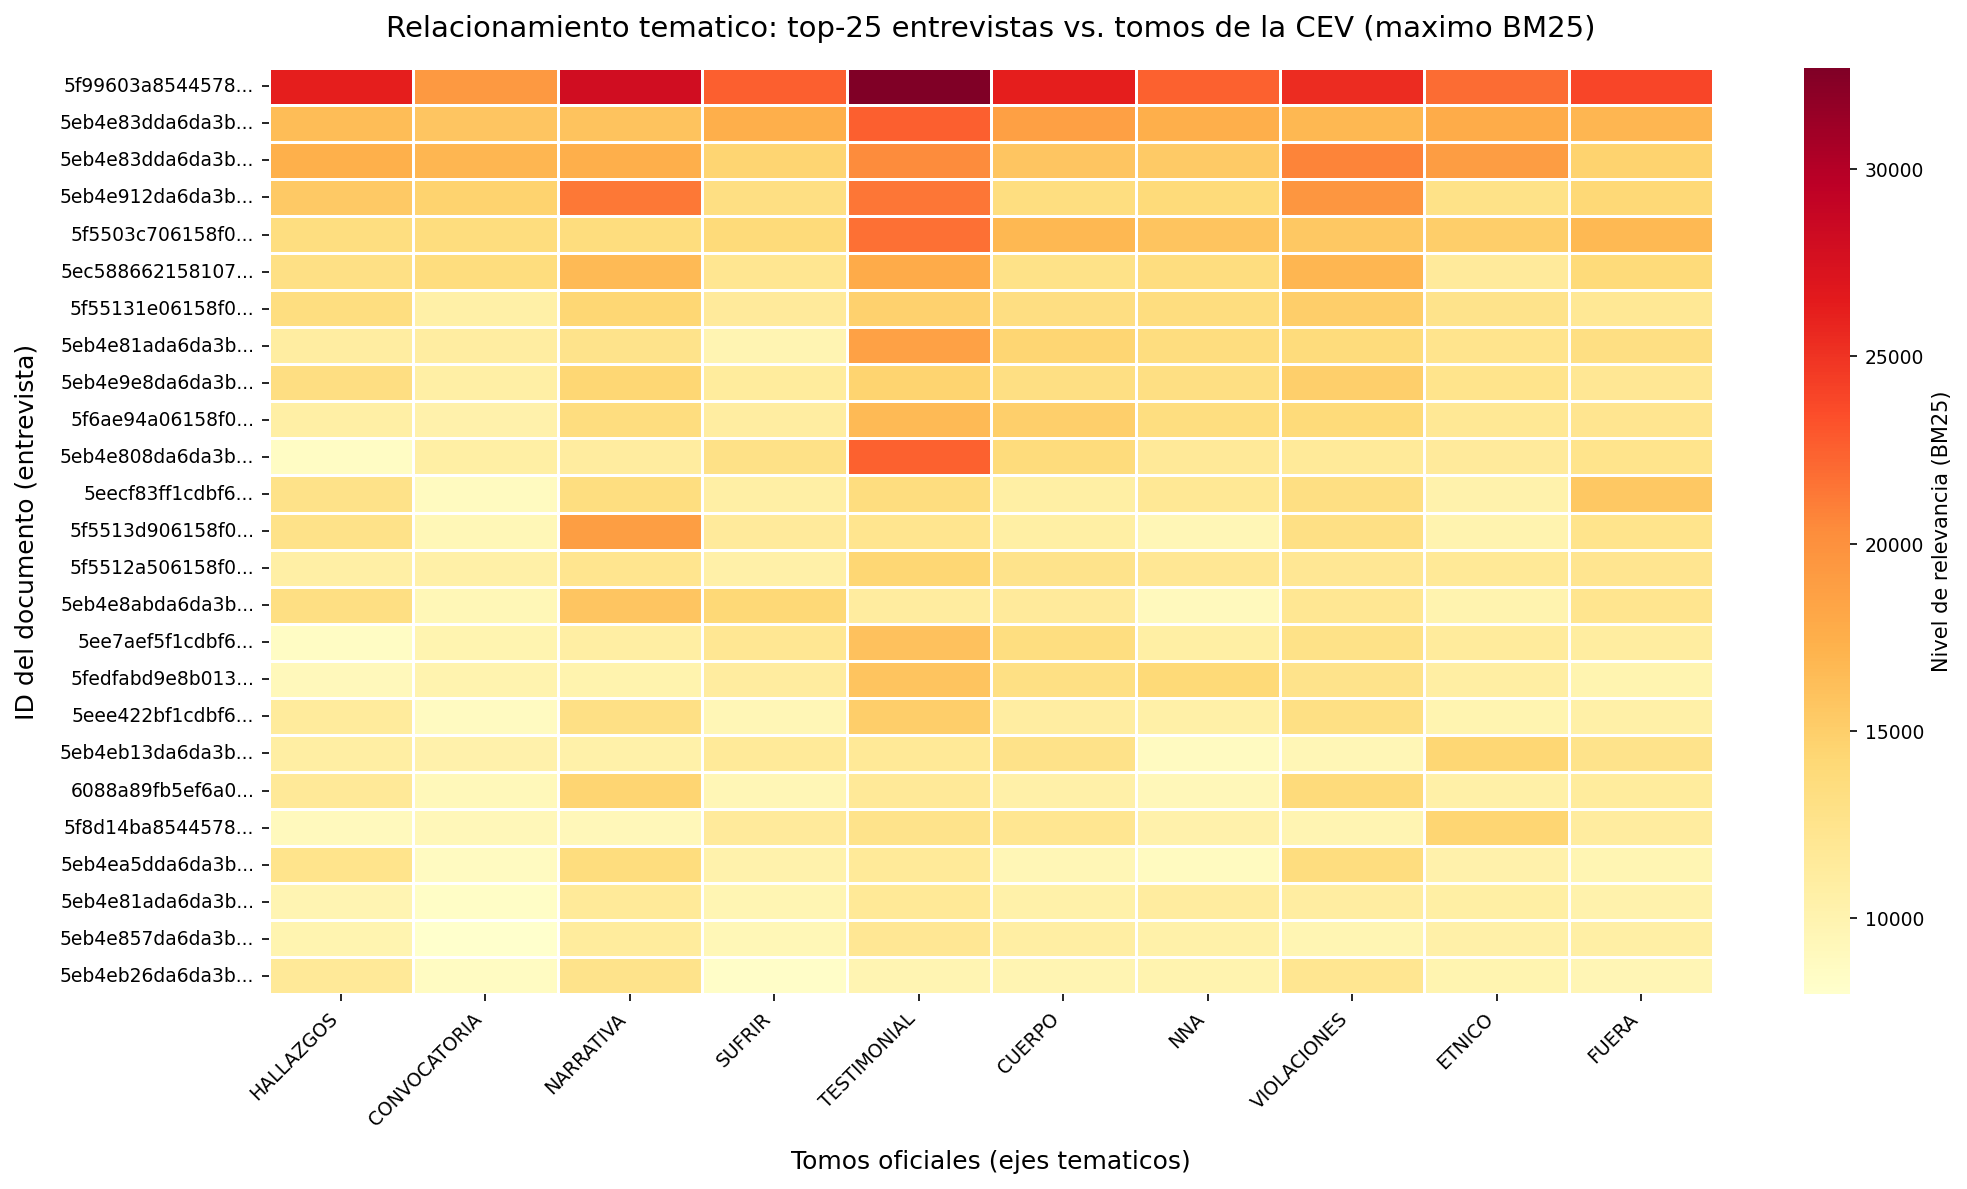
\includegraphics[width=0.62\textwidth]{figuras/heatmap_top25_entrevistas_tomos.png}
    \caption{Heatmap top-25 entrevistas $\times$ 10 tomos con el máximo score BM25 por celda. Las filas son las entrevistas con mayor suma de máximos por tomo. Conclusión: unas pocas entrevistas alcanzan afinidades muy altas (máximo 32.700,223 en TESTIMONIAL) y concentran su intensidad en pocos ejes temáticos; el patrón por documento hace visibles los vínculos fuertes que el promedio agregado 10$\times$10 difumina.}
    \label{fig:heatmap-top25}
\end{figure}

\subsection{Cuadro de vínculos}

El cuadro \texttt{resultados/vinculos\_entrevistas\_libros.csv} contiene \textbf{30 parejas} (3 por tomo) con el esquema \texttt{tomo, puesto, id\_doc, id\_segmento, score\_bm25, titulo\_segmento, fragmento\_entrevista, fragmento\_libro}: las dos últimas columnas incluyen $\approx$200 caracteres de lemas de contenido de cada parte para poder verificar cada vínculo sin releer los rankings completos, y la selección de 3 parejas por tomo garantiza que la inspección cualitativa cubra todos los tomos aunque la distribución del ranking esté sesgada. La Tabla~\ref{tab:vinculos} muestra la mejor pareja de cada tomo; las afinidades altas corresponden a solapes temáticos reconocibles (masacres, secuestro, pueblos étnicos, violencia sexual, persecución), lo que constituye la evidencia cualitativa de cierre del punto 5.

\begin{table}[htbp]
    \centering
    \caption{Mejor vínculo entrevista $\rightarrow$ segmento por tomo según BM25. Fuente: \texttt{resultados/vinculos\_entrevistas\_libros.csv}.}
    \small
    \setlength{\tabcolsep}{5pt}
    \begin{tabular}{l r p{8.4cm}}
    \toprule
    Tomo & Score BM25 & Título del segmento \\
    \midrule
    HALLAZGOS & 13.122,8 & La construcción histórica del actual modelo de seguridad y sus principales rasgos \\
    CONVOCATORIA & 6.296,5 & Primer paso del esclarecimiento: acoger la realidad de las víctimas \\
    NARRATIVA & 21.359,9 & 83. El body count o la doctrina Vietnam \\
    SUFRIR & 14.078,4 & Los obstáculos a la participación electoral y al derecho al voto \\
    TESTIMONIAL & \textbf{32.700,2} & Desafiar la realidad y los futuros deseados \\
    CUERPO & 8.072,2 & Afrontamientos de personas LGBTIQ+ víctimas del conflicto armado en Colombia \\
    NNA & 4.667,8 & Ataques a comunidades e instituciones educativas \\
    VIOLACIONES & 20.757,3 & ``No me pregunten porque yo no les sé darles respuesta'': torturas y tratos crueles \\
    ETNICO & 19.036,7 & Violencias, daños y resistencias de los pueblos étnicos en el conflicto armado \\
    FUERA & 15.560,5 & La persecución y la ausencia de protección en el marco de la responsabilidad del Estado \\
    \bottomrule
    \end{tabular}
    \label{tab:vinculos}
\end{table}


\section{P6 --- Evaluación crítica, conclusiones y mejoras futuras}\label{sec:p6}

\subsection{Conclusiones}

\textbf{P1.} Se extrajeron 917 segmentos y 2,27 M de palabras de los 10 tomos (mapeo TOC 91-100\,\%, cobertura 100\,\%, 0 solapes, 0 vacíos, 0\,\% fuera de banda) con una morfología documental explícita ---segmentos de sección en la banda 300-4.000 palabras--- que hace comparables los documentos entre tomos, y se normalizaron y preprocesaron 2.486 entrevistas ($-5{,}82$\,\% de caracteres; 40,35 M de tokens $\rightarrow$ 10,92 M de lemas; 8 categorías canónicas; 62 correcciones de lemas; 51 muletillas), preservando el contenido testimonial y unificando el vocabulario de ambos registros.

\textbf{P2.} Los libros son más diversos que las entrevistas incluso al controlar la longitud (TTR$_{m1000}$ 0,609 vs. 0,514; Yule K 31,8 vs. 38,7), el solapamiento de vocabulario es bajo (Jaccard 0,221) aunque la cobertura de tokens es alta y asimétrica (95,7\,\%/98,3\,\%), hay desajustes de registro relevantes (\textit{far/farc}) y 345 near-duplicados que se documentan sin eliminar. El EDA, además, fijó con evidencia los parámetros del modelo de P3 (\texttt{min\_df}, \texttt{max\_df}, bigramas y peso sublineal).

\textbf{P3.} El modelo TF-IDF, entrenado solo sobre la colección para evitar fuga de información, alcanza cobertura del 99,92\,\% y P@1 aceptable de 1,0, pero su P@1 estricto es 0,533 y su P@3 es 0,767: el primer resultado no siempre es el más específico (7/30 casos) y el sesgo TESTIMONIAL (76,77\,\%) es un efecto de dominio verificado. Los bigramas son la decisión de mayor impacto (54,8\,\% de coincidencia sin ellos).

\textbf{P4.} BM25 y Rocchio funcionan con auto-checks sintéticos en verde; BM25 comparte el 57,0\,\% del top-1 y el 65,7\,\% del conjunto top-5 con el base; Rocchio reordena el 29,9\,\% de los top-1 conservando el 100\,\% del inventario top-5, y su variante $k=3$ (24,0\,\% de top-1 distinto del base; 22,7\,\% del $k=5$) confirma que el tamaño del feedback importa y debe reportarse. Los tres métodos comparten el sesgo TESTIMONIAL, lo que refuerza su lectura como propiedad del dominio.

\textbf{P5.} La diagonal del heatmap (0,0725) supera a la afinidad fuera (0,0608) y a la media de fila en 10/10 grupos; el máximo de fila cae en la diagonal solo en 3/10, evidencia del sesgo de registro oral; los 30 vínculos con fragmentos muestran afinidades temáticas reconocibles y el heatmap top-25 conserva la intensidad individual que el promedio disuelve.

\textbf{P6.} El proceso es trazable de extremo a extremo: \texttt{resultados/metricas.json} por fase, semilla 42, auditoría sin PII en los corpus finales, 51 pruebas pytest aprobadas y ruff 0.

\subsection{Limitaciones}

(a) \textbf{Sin gold estándar}: la evaluación es proxy sobre 30 pares etiquetados por el equipo, sin acuerdo inter-etiquetador ni P@$k$ externo para BM25 ni Rocchio; las cifras deben leerse como indicios de plausibilidad y no como una comparación contra una referencia independiente. (b) \textbf{Lematizador imperfecto} en voseo y pretéritos, mitigado con 62 correcciones en consumo que cubren los casos observados, pero que no constituyen una solución general. (c) \textbf{345 near-duplicados} replican rankings y sobreestiman la cobertura; al conservarlos por integridad del corpus, la cobertura del 99,92\,\% debe interpretarse como cobertura sobre el corpus oficial, no sobre un corpus deduplicado. (d) \textbf{El matching léxico no discrimina} hechos o poblaciones específicas: compite por solape temático amplio, de modo que un score alto indica afinidad de vocabulario, no correspondencia factual verificada. (e) \textbf{El intermedio} \texttt{entrevistas\_normalizadas.jsonl} conserva PII hablada y no es distribuible; los corpus finales están limpios y \texttt{data/raw/} permanece intacto, por lo que la distribución se apoya en los 3 insumos y en la regeneración automática. (f) La longitud de BM25 se mide en \textbf{términos del vocabulario} ($avgdl$ 1.466,26), no en lemas de contenido (1.007,5), una precisión necesaria para reproducir el cálculo y para no confundir la escala de la fórmula con la estadística descriptiva del corpus. (g) La agrupación del heatmap \textbf{hereda el sesgo TESTIMONIAL}: mide coherencia entre asignación y afinidad, no corrección de los vínculos.

\subsection{Mejoras futuras}

(i) \textbf{BM25 tuneado} con búsqueda de $k_1\in[0{,}9;2{,}0]$ y $b\in[0{,}3;1{,}0]$, viable ahora que existe una implementación verificada, aunque requerirá un gold o al menos una muestra mayor para elegir la configuración sin sobreajustar. (ii) \textbf{Embeddings y \textit{reranking}} supervisado del top-$k$ para superar el techo del solape léxico \cite{valentini2024messirve}: los modelos densos permiten recuperar paráfrasis que TF-IDF no alcanza, a costa de perder la trazabilidad término a término. (iii) \textbf{Gold estándar externo} con acuerdo inter-etiquetador, que convertiría las métricas proxy en métricas comparables. (iv) \textbf{Eliminación o agrupación de near-duplicados} para no inflar la cobertura. (v) \textbf{Enrutamiento por tomo} (clasificador previo) para corregir el prior TESTIMONIAL. (vi) \textbf{Cambio de hablante, \textit{chunking}} de entrevistas largas y limpieza fina de \textit{running heads}. (vii) \textbf{Expansión semántica} con el tesauro CEV, hoy reservado para análisis cualitativo.


\section{Entregables y reproducibilidad}\label{sec:entregables}

\subsection{Entregables del taller}

La Tabla~\ref{tab:entregables} mapea cada entregable del enunciado con su artefacto y su ruta en el repositorio. El artefacto central es el \textbf{notebook único} \texttt{notebooks/Taller\_4\_IR\_CEV.ipynb} (125 celdas), que integra los seis puntos y fusiona los aportes de los dos desarrollos paralelos del equipo (el base y la versión 2, retirada al quedar integrada); se optó por una versión única para que exista una sola fuente de verdad reproducible y para que ninguna salida dependa de un cuaderno que ya no se mantiene. El informe markdown y este informe LaTeX son sus documentos acompañantes.

\begin{table}[htbp]
    \centering
    \caption{Entregables del enunciado y su ubicación en el repositorio.}
    \footnotesize
    \setlength{\tabcolsep}{4pt}
    \begin{tabular}{>{\raggedright\arraybackslash}p{3.0cm} >{\raggedright\arraybackslash}p{4.6cm} >{\raggedright\arraybackslash}p{7.0cm}}
    \toprule
    Entregable & Artefacto & Ruta \\
    \midrule
    Corpus extraído y preprocesado & Crudo sin tocar y corpus limpios & \texttt{data/raw/}; \texttt{data/corpus/segmentos\_libros.jsonl} (917); \texttt{entrevistas\_normalizadas.jsonl} (2.486); \texttt{data/corpus/preprocesado/} \\
    Análisis exploratorio & Informe, 18 CSV y 14 figuras & \texttt{resultados/eda/}; \texttt{imagenes/eda\_*.png} \\
    Modelo de IR (código y reporte) & Script, notebook y reporte JSON & \texttt{experimentos/experimento\_1\_tfidf\_base.py}; \texttt{resultados/ir\_tfidf\_report.json}; \texttt{ranking\_top5.csv} \\
    Funciones de métricas & BM25 y Rocchio manuales + rankings & Sección 03b del notebook; \texttt{ranking\_bm25.csv}; \texttt{ranking\_rocchio.csv}; \texttt{ranking\_rocchio\_k3.csv} \\
    Comparación entrevistas--libros & Cuadro y heatmaps & \texttt{resultados/vinculos\_entrevistas\_libros.csv}; \texttt{heatmap\_tomos.csv}; \texttt{heatmap\_top25.csv}; figuras \texttt{heatmap\_*.png} \\
    Informe final & Markdown y LaTeX & \texttt{informe/informe\_taller4.md}; \texttt{informe\_latex/main.tex} (este documento) \\
    Notebook entregable & Flujo completo reproducible & \texttt{notebooks/Taller\_4\_IR\_CEV.ipynb} (125 celdas) \\
    \bottomrule
    \end{tabular}
    \label{tab:entregables}
\end{table}

\subsection{Cómo ejecutar el notebook con solo 3 insumos}

El notebook es independiente: para ejecutarlo de extremo a extremo solo requiere \textbf{tres insumos descargados manualmente} a \texttt{data/raw/}: (1) el dataset de entrevistas \texttt{entrevistas\_all\_2023-03-21\_14-24\_05.json} ($\approx$231 MB); (2) el zip de libros de la CEV \texttt{books-*.zip} (o la carpeta \texttt{books/} con los PDF, $\approx$300 MB); y (3) el tesauro \texttt{Resource-tesauro.rdf} ($\approx$5 MB). Todo lo demás ---segmentos, entrevistas normalizadas, lemas, tokens, CSVs y figuras del EDA--- lo \textbf{genera} la sección ``Sec 0b --- Regeneración'' con \texttt{REGEN\_AUTOMATICO=True} (por defecto), porque la configuración curada (muletillas, correcciones, ruido y parámetros TF-IDF) viaja embebida como constantes. Esta decisión de diseño evita dos problemas frecuentes en la entrega de cuadernos: depender de rutas locales inexistentes y requerir datos derivados que no siempre se pueden redistribuir. \texttt{config/}, \texttt{resultados/} e \texttt{imagenes/} son opcionales: si existen, el notebook los usa como verificación o respaldo visual; si se borran, no se rompe.

\textbf{Ejecución local.} Basta el entorno virtual del proyecto (\texttt{pandas}, \texttt{scikit-learn}, \texttt{spacy} con \texttt{es\_core\_news\_md}, \texttt{matplotlib}, \texttt{seaborn}, \texttt{wordcloud} y \texttt{nbclient}; \texttt{poppler-utils} solo para regenerar la extracción de PDF) y ejecutar todas las celdas. La primera corrida sin cachés tarda 15-60 minutos (libros 5-15 min; spaCy 10-40 min), tiempos compatibles con una sesión de trabajo y con la política de regeneración automática. \textbf{Ejecución en Colab.} Se sube la carpeta \texttt{TALLER-4} a \texttt{/content} (o se deja como \texttt{/content/PLN-main/TALLER-4}), o se activa \texttt{AUTO\_DESCARGAR\_REPO=True}; el notebook localiza la raíz por marcador, variable de entorno \texttt{TALLER4\_ROOT} o rutas típicas de Colab, de modo que el mismo cuaderno funciona en local y en la nube sin editar rutas. El pipeline por fases equivalente es \texttt{01\_extraer\_libros.py} $\rightarrow$ \texttt{02\_preprocesar.py} $\rightarrow$ \texttt{03\_eda.py} $\rightarrow$ \texttt{experimento\_1\_tfidf\_base.py} $\rightarrow$ \texttt{04\_evaluar\_muestra.py}.

\textbf{Evidencia de independencia.} La verificación se hizo en cuatro frentes, pensados para cubrir tanto la ejecución real como la reproducibilidad de la configuración: (i) ejecución aislada de extremo a extremo con solo el \texttt{.ipynb} y los 3 insumos, con 0 errores en 922 s ($\approx$15,4 min), que demuestra que no hay dependencia de caches; (ii) sandbox de pruebas sin \texttt{config/}, \texttt{resultados/}, \texttt{imagenes/} ni \texttt{scripts/} (65,8 s) con 51 pruebas pytest aprobadas; (iii) corrida completa en el repositorio en 61,7 s con 0 errores y modelo base idéntico al oficial en 2.484/2.484 top-1 (TESTIMONIAL 76,77\,\%; variantes 54,8/84,6/96,6; P@1 0,5333/1,0 y P@3 0,7667/1,0), que confirma la paridad entre el notebook y los artefactos publicados; y (iv) ruff 0. El detalle está en \texttt{plan/verificacion\_independencia\_notebook.md} y la autoevaluación de la rúbrica en \texttt{plan/verificacion\_rubrica.md}.


\nocite{*}
\bibliographystyle{apalike}
{\footnotesize\sloppy
\setlength{\itemsep}{1pt plus 0.2ex}
\setlength{\parsep}{0pt}
\bibliography{references}}

\end{document}
